% -----------------------------------------------------------------------
% Python Tutorial
% WS 18/19
% -----------------------------------------------------------------------
\documentclass[enabledeprecatedfontcommands, fontsize=12pt,
     open=right, a4paper,
     twoside, DIV=11,
     abstractoff,
     headsepline,
     numbers=noenddot,
     BCOR=15mm,
     headings=standardclasses,
     headings=big]{scrbook}
\KOMAoptions{cleardoublepage=empty}
% Header f�r Variablen
% Variablen
\newcommand{\theSemester}{WS18/19}
% Variable f�r die Vorlesung
\newcommand{\theProject}{Informatik studieren in der digitalen Gesellschaft\\Collaborative Writing}
% Variable f�r den Studiengang
\newcommand{\theTitle}{Python}
% Variable f�r den Hochschul-Namen
\newcommand{\theSchool}{Hochschule Kaiserslautern}
% Variable f�r den Dozenten
\newcommand{\theAuthor}{
    Julian  Bernhart,
    Manfred Brill,
    Eric Brunk,
    Mathias Fedder,
    Robin Marc Guth,
    Rainer Haffner,
    Matthias Haselmaier,
    Kathrin Hentschel,
    Fabian Kalweit,
    Kevin Konrad,
    Philipp Lauer,
    Miriam Lohm�ller,
    Pascal Pries,
    Anatoli Sch�fer,
    Denis Schlusche,
    Christoph Seibel,
    Marc Zintel
}

%
% ----------------------------------------------------------------------------------------------
% Vorlage f�r Dokumentation auf LaTeX-Basis im Projekt InfoStuDi
% --------------------------------------------------------------------------------------------
\usepackage{mb}
 \usepackage{mbmath}
\usepackage{textcomp}
% Array-Paket f�r mehr Kontrolle der Tabellen
\usepackage{array}
% ifthen f�r Ein- und Ausblenden der L�sungen.
\usepackage{ifthen}
% Paket f�r Postscript Pi-Fonts
\usepackage{pifont}
% PSTricks
%\usepackage{pstricks}
% Paket f�r das einfache Umdefinieren von Listen
\usepackage[shortlabels]{enumitem}
% Alphabetischer Index
\usepackage{imakeidx}
\makeindex[title=Index,columns=2,options=-s german,intoc]
% Header und Footer mit KomaScript
\usepackage[automark, headsepline]{scrlayer-scrpage}
%
% Header f�r Werkzeuge, Begriffe aus dem Software-Management
\input{variablen}
% Farben
\input{colors}
% Koordinatensysteme und andere Makros
\input{coordinateSystems}
% Standardverzeichnis f�r das Basisverzeichnis der Bilder
%
\newcommand{\imagePath}{./images}
%
\raggedbottom
\setlength{\parskip}{2.0ex}
\setlength{\parindent}{0.0cm}
%% Verhindert Schusterjungen und Hurenkinder
\clubpenalty = 10000
\widowpenalty = 10000 \displaywidowpenalty = 10000
%
\setcounter{secnumdepth}{2}
\setcounter{tocdepth}{2}
%
\pagestyle{scrheadings}
\clearscrheadfoot
% Thema des Dokuments in die Kopfzeile
\ihead{\headmark}
\ohead[]{\pagemark}
\chead{}
\pagestyle{scrheadings}
% Abst�nde zwischen Caption und Bild/Tabelle
\setlength\abovecaptionskip          {0.4em}
\setlength\belowcaptionskip          {0.2em}
% Anteil der Grafiken h�her auf jeder Seite!
\renewcommand{\textfraction}{0.001}
\renewcommand{\topfraction}{0.99}
% Literatur-Stil
\bibliographystyle{geralpha}
% Listingspaket
\usepackage{listings}
\lstloadlanguages{Java}
\lstset{language=Java}
\definecolor{lstback}{gray}{0.85}
\lstset{backgroundcolor=\color{lstback}}
\lstset{extendedchars=true}
\lstset{showstringspaces = false}
\lstset{basicstyle = \ttfamily \small}
%% listings mit listings.sty
%
% Kommando f�r den Flattersatz bei nebeneinander liegenden Abbildungen
\newcommand{\flatter}{\setlength{\rightskip}{0pt plus 2cm}}
%
% Schritte in einer Aufz�hlung, daf�r einen Z�hler (schritt) und die Umgebung
% schritte definieren.
\newcounter{schritt}
\newenvironment{schritte}%
{\begin{list}%
{Schritt \arabic{schritt}:}%
{\usecounter{schritt}\settowidth{\labelwidth}{Schritt 1:}%
\setlength{\leftmargin}{\labelwidth}\addtolength\leftmargin{\labelsep}%
\parsep0.0ex\partopsep-0.3ex\itemsep2pt\topsep0.0ex}}{\end{list}}
% Dateinamen f�r interne Musterl�sungen
\newcommand{\filename}[1]{%
\ifthenelse{\boolean{solutions}}{\framebox[50mm]{\parbox{40mm}{\textbf #1}}\vspace{6pt}}{}}
%   Taste
\newcommand{\taste}[1]{\small\textsf{#1}\normalsize}
%   gesch�tzte Namen (NICHT in chapter, section usw. verwenden!)
\newcommand{\name}[1]{\textsl{#1}}
%   Fachbegriffe/Erkl�rung von Abk�rzungen
\newcommand{\begriff}[1]{\index{#1}\textit{#1}}
%
\newcommand{\algorithmus}[2]{%
\vspace{4pt}\fboxsep 1mm \framebox[140mm]
{\parbox{135mm}{{\textbf{#1}}\vspace{2pt}#2}}\vspace{4pt}}
%
%   Dateinamen/Pfade
\newcommand{\datei}[1]{\texttt{#1}\normalsize}
%   Tip (in einer Box)
\newcommand{\tip}[1]{%
\vspace{4pt}\fboxsep 1mm \framebox[140mm]
{\parbox{135mm}{{\textbf{Tipp}}:\\ #1}}\vspace{4pt}}

%Achtung in einer Box
\newcommand{\warning}[1]{%
	\vspace{4pt}\fboxsep 1mm \framebox[140mm]
	{\parbox{135mm}{{\textbf{Achtung}}:\\ #1}}\vspace{4pt}}
%

%
%   Reflektion (in einer Box)
%
\newcommand{\reflection}[1]{
\begin{quote}\fboxsep 3mm\framebox[140mm][c]{\parbox{130mm}{{\textbf{Reflektion}:\\}#1}}\end{quote}}
%
%   Angabe, was die Studierenden lesen sollen (in einer Box)

\newcommand{\lesen}[1]{%
\begin{minipage}[c]{2.5cm}
\centering
\includegraphics[width=2cm]{\imagePath/Misc/buchicon}%
\end{minipage}%
\begin{minipage}[t]{12cm}%
#1%
\end{minipage}}
%
%   Angabe im Begleittext, was die Studierenden lesen sollen (in einer Box)
%   Dieses Icon wird f�r Angaben verwendet, die nicht verpflichtend zu lesen
%   sind. Also "nice-to-have", "wenn sie noch Zeit haben".
\newcommand{\vertiefen}[1]{%
\begin{minipage}[b]{2.5cm}
\centering
\includegraphics[width=2cm]{\imagePath/Misc/reading}%
\end{minipage}%
\begin{minipage}[b\newcommand{\firefox}{\texttt{Mozilla Firefox}}
\newcommand{\kde}{\texttt{KDE}}]{12cm}%
#1%
\end{minipage}}
%
% Jetzt kommt die Definition der Kontrollfrage; die Nummerierung
% f�r das ganze erhalten wir mit Hilfe von \item{\kontroll}.
%
% Ein Counter f�r die Kontrollfragen. Wir z�hlen diesen Counter selbst hoch
% mit einem entsprechenden Kommando, das wir in \item verwenden.
% 1
\newcounter{kontrollCounter}[section]
\newcommand{\kontroll}[0]{
    \refstepcounter{kontrollCounter}
    % Kapitelnummer.Z�hler f�r das Item
    \arabic{chapter}.\arabic{kontrollCounter}
    % Das Label ist bis auf weiteres "kontrolle:Kapitelnummer:kontrollcounter
    \label{kontrolle:\arabic{chapter}:\arabic{kontrollCounter}}
}
% Jetzt kommt die Definition der Kontrollfrage; die Nummerierung
% f�r das ganze erhalten wir mit Hilfe von \item{\kontroll}.
\newcommand{\kontrollfrage}[1]{%
\begin{minipage}[c]{1.85cm}
\huge{\ding{46}}%
\end{minipage}%
\begin{minipage}[t]{12cm}%
\begin{itemize}#1%
\end{itemize}%
\end{minipage}}
%
% Einblenden von Musterl�sungen
%
% Schalter f�r das ein- und ausblenden der L�sungen
\newboolean{solutions}
%
% Theorem-Umgebung f�r die �bungsaufgaben
% Wichtig: alle Attribute einstellen, dann die neue
% theorem-Umgebung mit newtheorem definieren!
% Oder, wie hier, durch das Einschlie�en in {}
%
{
% Zeilenumbruch bei Aufgaben-�berschrift
\theoremstyle{break}
% "Normaler" Font im Text
\theorembodyfont{\normalfont}
% Kapitelweise neu nummerieren
% 2
\newtheorem{auftitle}{Aufgabe}[section]
}
%
% Definition f�r die Kennzeichnung der �bungsaufgaben
%
\newcommand{\uebung}{%
\vspace*{11pt}%
\begin{tabular}{@{}p{2.25cm}@{}p{11.7cm}}%
\huge{\ding{45}}&\Large{\textbf{�bungsaufgaben}}%
\end{tabular}%
}
% Ein Counter f�r die �bungsaufgaben. Wir z�hlen diesen Counter selbst hoch
% mit einem entsprechenden Kommando, das wir in \item verwenden.
% 3
\newcounter{aufgabenCounter}[section]
\newcommand{\auf}[0]{
    \refstepcounter{aufgabenCounter}
    % Kapitelnummer.Z�hler f�r das Item
    \arabic{chapter}.\arabic{aufgabenCounter}
}
% Der Text der Aufgaben steht im Ordner ./exercises/tasks/aufgabenstellungen,
% so k�nnen wir die Dateien aus der Veranstaltung
% Wahrscheinlichkeitsrechnung und Statistik verwenden; und die neuen
% Aufgaben gehen in den allgemeinen Fundus ein.
%

% Umgebungen f�r Satz, Definition, Beweis, ... . Wir orientieren uns am Mathematik-Buch,
% dort gab es diese Umgebungen auch schon. Im Grunde sind das einfach
% wieder theorem-Umgebungen.
{
\setlength\theorempreskipamount{5pt plus 3pt minus 1.5pt}
\setlength\theorempostskipamount{5pt plus 1pt minus 1pt}
% "Normaler" Font im Text
\theorembodyfont{\normalfont}
% Die Namen sind so gew�hlt, dass sie kompatibel zu Beamer sind; dann k�nnen
% wir den Text aus Folien kopieren und umgekehrt auch.
% 4
\newtheorem{Satz}{Satz}[section]
\newtheorem{Fakt}{Fakt}[section]
\newtheorem{Definition}{Definition}[section]
}
%
{
\setlength\theorempreskipamount{8pt plus 3pt minus 1.5pt}
\setlength\theorempostskipamount{5pt plus 1pt minus 1pt}
\theoremstyle{break}
% "Normaler" Font im Text
\theorembodyfont{\normalfont}
\newtheorem{datensatz}{Datensatz}
}
% Text mit Pfad
\newcommand{\aufgabentext}[1]{\renewcommand{\labelenumi}{\alph{enumi})}\auftitle\label{#1}\input{./exercises/tasks/#1}}
% Funktion f�r die L�sungs-Hinweise f�r eine Aufgabe. Der Text
% steht analog zu den �bungsaufgaben im Ordner tasks/solutions.
\newcommand{\hinweistext}[1]{\renewcommand{\labelenumi}{\alph{enumi})}\input{./exercises/solutions/#1}}
% Und jetzt die Funktionen, die wir im Text aufrufen
\newcommand{\aufgabe}[1]{\aufgabentext{#1}}
% L�sungshinweise im Anhang
\newcommand{\hinweis}[1]{\subsubsection*{Aufgabe \ref{#1}} \hinweistext{#1}}
%
% Datensatz-Texte und Daten in eigener Datei
\newcommand{\dataset}[1]{\begin{datensatz}\label{#1}\input{./exercises/datasets/#1}\end{datensatz}}
% Teilaufgaben alphabetisch nummerieren
\renewcommand{\labelenumi}{\arabic{enumi})}
%
% Marginalien
%
\newcommand{\randnotiz}[1]{\marginpar{\small{\textbf{#1}}}}
%
% Gabelschl�ssel als Marginalie und Hinweis auf Praxisbezug
\newcommand{\praxisbezug}[0]{\randnotiz{\includegraphics[width=1cm]{\imagePath/Misc/gabel}}}
%
% alert aus beamer-Folien zu emph machen
%
\newcommand{\alert}[1]{\emph{#1}}
%
%
\newcommand{\titelseite}[1]{%
% Titelseite
\pagenumbering{roman}%
\thispagestyle{empty}%
\begin{titlepage}%
% Volle Zeilenbreite verwenden!
\centering%
\vspace*{2cm}%

\Huge{#1}\\\vspace*{0.5cm}%

\vspace*{10cm}%

\Large{\theAuthor{}}%

\Large{\theProject{}}%

\Large{\theSchool{}}%
\end{titlepage}}

% Titelseite mit zus�tzlicher Grafik
%
% Das obligatorische Argument ist der Titel des Dokuments.
% Als Default wird das Logo der Stochastik-Veranstaltung als Titelbild
% verwendet. Mit Hilfe eines optionalen Arguments kann
% ein anderes Bild verwendet werden!
% Beispiel: \titelseite[\imagePath/misc/ameise]{Das Liebesleben der Ameisen}
% Aufruf mit Standardbild:
% \titelseite{Das Liebesleben der Ameisen}
%
\newcommand{\titelseiteMitBild}[2][\imagePath/logos/python]{%
%% Titelseite
\pagenumbering{roman}%
\thispagestyle{empty}%
\begin{titlepage}%
% Volle Zeilenbreite verwenden!
\centering%
\vspace*{0.5cm}%

\Huge{#2}\\\vspace*{0.5cm}%

\vspace*{3.0cm}%
\includegraphics[height=6cm]{#1}%

\vspace*{3.0cm}%
\Large{\theAuthor{}}%

\Large{\theProject{}}%

\Large{\theSchool{}}%
\end{titlepage}} 
%
% Schalter f�r das Ein- und Ausblenden der L�sungen
\setboolean{solutions}{true}
%
\input{pdfsetup}
%
% Beginn Dokument
%
\begin{document}
\titelseiteMitBild{\theTitle{}}
%
% Vorwort
%
% !TeX root = ../pythonTutorial.tex
\chapter*{Vorwort}
Das vom Stifterverband gef�rderte Projekt \glqq Informatik studieren in der digitalen Gesellschaft (InfoStuDi)\grqq{}
erprobt und evaluiert neue Lehr-, Lern- und Pr�fungsformen in den Informatik-Studieng�ngen im Fachbereich Informatik und Mikrosystemtechnik der Hochschule Kaiserslautern. 
Studieng�nge an einer Hochschule f�r
angewandte Wissenschaften bereiten die Studierenden auf die sp�tere Arbeitswelt vor. 
Diese Arbeitswelt
wird von zeitlich und �rtlich ungebundenem Arbeiten gepr�gt sein.

Im Teilprojekt \glqq Collaborative Writing\grqq{} wurde eine neue Form einer Lehrveranstaltung erprobt.
Ein Team aus Studierenden und Lehrenden verfasst ein Dokument zu einem Thema der Informatik. 
Dabei wird neben der Produktion von Texten auch Software entstehen.  
Die Produktion des vorliegenden Dokuments
zum Thema Python wurde wie ein gro�es agiles Software-Projekt organisiert. 
Drei Sprints wurden durchgef�hrt, das Team organisierte sich selbst. Werkzeuge wie \LaTeX{}, Git oder Jenkins wurden eingesetzt.
Die Studierenden waren nicht nur Autoren, sondern auch Fachlektoren, Software-Entwickler und f�r die Qualit�t des Gesamtergebnisses mit verantwortlich.

Dieses Projekt w�re nicht zustande gekommen ohne die Studierenden, die sich auf dieses Abenteuer im Rahmen
der Lehrveranstaltung \glqq Aktuelle Themen aus Forschung und Praxis\grqq{} im Masterstudiengang Informatik eingelassen haben. An dieser Stelle ein herzliches \glqq Danke Sch�n!\grqq{} f�r das Vertrauen und den Mut, sich auf diese Form einer
Lehrveranstaltung einzulassen.
Miriam Lohm�ller brachte ihre Erfahrung aus dem Verlagswesen ein und hat die von den Studierenden verfassten
Texte lektoriert. Fabian Kalweit hat das fachliche Lektorat unterst�tzt und insbesondere das Backend in GitHub
organisiert und gestaltet. 
\vspace{\baselineskip}
\begin{flushright}\noindent
Zweibr�cken, im Januar 2019\hfill

\hfill {\it Manfred  Brill}
\end{flushright}


%
% Inhaltsverzeichnis
%
\tableofcontents
\clearevenpage
\pagenumbering{arabic}
%
%
%

%\uebungZwei{beispielAufgabe1}{grundlagen01}{grundlagen02}

% !TeX root = ../pythonTutorial.tex
\chapter{Grundlagen}

\section{Was ist Python?} %TODO ADD INFORMATION AND INTRODUCTION
\label{grundlagen:sec:WasIstPython}
Die Programmiersprache Python wurde Anfang der 1990er Jahre von Guido van Rossum entwickelt.
Der Name der Sprache beruht auf der Komikergruppe  Monty Python.
Hierzu lassen sich auch zahlreiche Anspielung in der Dokumentation von Python finden.
Python wurde mit dem Ziel gr��ter Einfachheit sowie �bersichtlichkeit entworfen.
Dies wird nicht zuletzt durch die Gr��e �bersichtlichkeit in der Standardbibliothek versucht zu erreichen sondern auch durch die Modulare Erweiterbarkeit.
Im Folgenden wird die Programmiersprache Python in der Version 3 behandelt.

\section{Installation}
\randnotiz{Installation}
\label{grundlagen:sec:Installtion}
Python kann auf der Webseite \url{https://www.python.org} f�r eine Vielzahl von Betriebssystemen bezogen werden. 
Es stehen 32- und 64-Bit Versionen zur Verf�gung. 
Nach dem Start des Installationsassistenten f�hrt er den Nutzer durch den Installationsprozess. 
Der Ablauf der Installation unterscheidet sich zwischen den Betriebssystemen nur gering bis gar nicht.
Nach erfolgreichem Abschluss stehen dem Anwender verschiedene Programme und zur Arbeit mit Python zur Verf�gung.
Im vom Nutzer gew�hlten Installationsverzeichnis befinden sich nun folgende Programme: 
\begin{description}
    \item[\textit{IDLE}] Standard IDE\footnote{Integrated Development Environment} f�r Python
    \item[Python] Standard Konsolen Interpreter
    \item[Pythonw] Standard Interpreter ohne Konsolenausgabe
\end{description}
Diese Programme reichen aus, um Code mit Python zu entwickeln. 
Der Python Interpreter kann nun in der Konsole mit dem Befehl ''python'' aufgerufen werden. 
Die folgenden Abschnitte beschreiben Besonderheiten bei der Installation auf einzelnen Betriebssystemen. 
\subsection{Hinweis zur Installation unter Windows}
\label{grundlagen:sec:InstallationWindows}
Windows Nutzer m�ssen die Systemvariable f�r Python im Installationsassistenten hinzuf�gen lassen. 
Andernfalls kann Python nur im Installationsverzeichnis bzw. durch die Angabe des kompletten Pfades aufgerufen werden. 
In Abbildung \ref{grundlagen:img:InstallationWindows} ist die notwendige Auswahl zu sehen. 
\begin{figure}[ht]
\centering
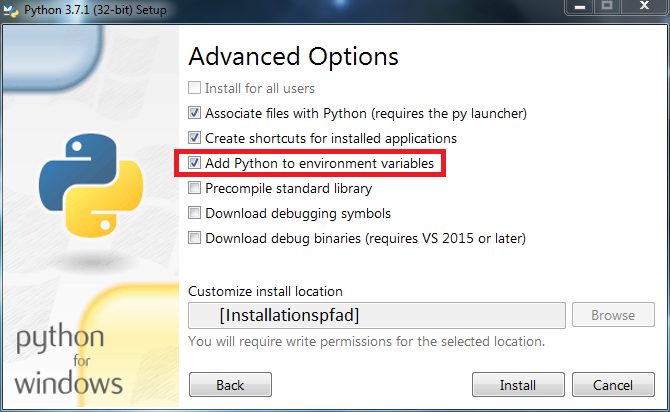
\includegraphics[scale=0.5]{images/InstallationWindows.png}
\caption{Start des Installationsassistenten}
\label{grundlagen:img:InstallationWindows}
\end{figure}
%
\subsection{Hinweis zur Installation unter Mac}
\label{grundlagen:sec:InstallationMac}
Im Folgenden wird die Installation unter macOS X gezeigt.

\begin{figure}[ht]
	\centering
	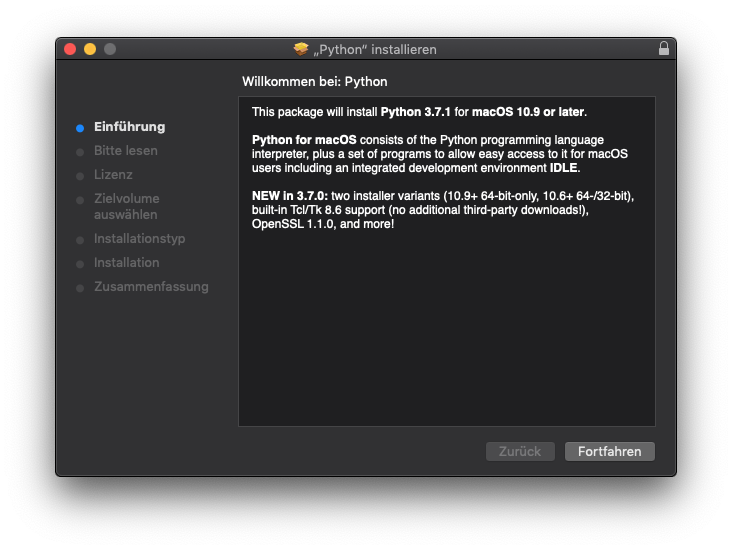
\includegraphics[scale=0.5]{images/InstallationMac.png} 
	\caption{Start des Installationsassistenten}
	\label{grundlagen:img:InstallationMac}
\end{figure}
Nach Ende der Installation befindet sich der Python Ordner im Finder (Dateiexplorer).

\begin{figure}[ht]
	\centering
	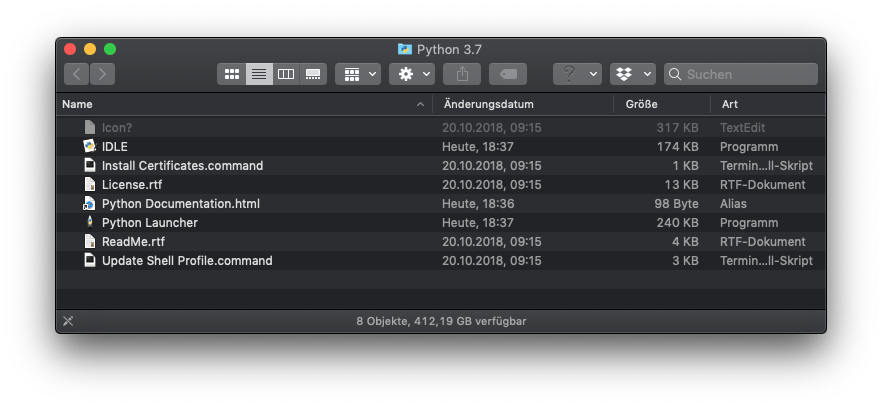
\includegraphics[scale=0.5]{images/PythonFinder.png} 
	\caption{Fertige Installation}
	\label{grundlagen:img:FinishInstall}
\end{figure}
Zuletzt wurde durch den Assistent unter /Library/Frameworks/Python.framework noch das Python Framework abgelegt.
Ohne dieses w�re das Arbeiten mit Python unter Mac nicht m�glich.

\subsection{Hinweis zur Installation unter Linux(Ubuntu)}
\label{grundlagen:sec:InstallationLinux}
Im Folgenden wird die Installation f�r Ubuntu Version 18.04.1 LTS erl�utert.
Im Gegensatz zu den anderen Betriebssystemen, wird hier von Haus aus ein Python Interpreter in der Version 3.6.6 mitgeliefert, jedoch nicht die Standard Entwicklungsumgebung IDLE.
Diese kann �ber das Paket \textit{IDLE} nachtr�glich installiert werden.
Sollte trotzdem noch kein Python vorhanden sein, durch den folgenden Befehl die Installation manuell angesto�en werden.

\begin{lstlisting}[language=BASH, label={grundlagen:lst:InstallationLinux}]
sudo apt-get install python3 python-doc
\end{lstlisting}

Diese Installation umfasst unter anderem auch die Dokumentation von Python.
Nach Abschluss der Installationsroutine kann wie mit jedem anderen Betriebssystem mit Python gearbeitet werden.

%TODO Skript versus Programm
\section{Python Interpreter} %WIP ROGU 
\label{grundlagen:sec:Interpreter}
%TODO ADD LINKS TO OTHER SECTIONS %WHAT IS PYTHON CODE?
Die einfachste M�glichkeit, Python Code auszuf�hren, ist direkte �bergabe des Codes an den sogenannten Python Interpreter. 
Dabei handelt es sich um eine Konsolenanwendung, welche Code ausf�hren und gegebenenfalls auftretende Ergebnisse ausgeben kann. 
Dabei kann ein Nutzer den Code entweder direkt in die Konsole eingeben oder diesen aus einer Datei auslesen lassen. 
Wie bei anderen Programmiersprachen auch, stehen f�r Python verschiedene IDEs zur Verf�gung, welche in Kapitel \ref{} behandelt werden. 
F�r die ersten Versuche mit Python reicht der Interpreter jedoch v�llig aus. Dieser wird standardm��ig mit Python installiert.

In Abbildung \ref{grundlagen:img:Interpreter} ist der Interpreter zu sehen. 
Zus�tzlich zur Version werden auch noch der Herausgeber von Python, sowie die Uhrzeit angezeigt.
Bereits jetzt kann erster Code ausgef�hrt werden.
Im Folgenden werden zu einzelnen Bestandteilen von Python Beispiele beigef�gt, welche leicht im Interpreter ausf�hrbar sind. Es wird dem Leser empfohlen, diese zum besseren Verst�ndnis nachzuvollziehen, falls m�glich durch eigenst�ndiges Ausprobieren.

\begin{figure}[ht]
	\centering
	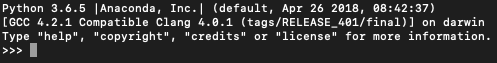
\includegraphics[width=0.8\textwidth]{images/Interpreter.png} 
	\caption{Ansicht nach Start des Interpreters}
	\label{grundlagen:img:Interpreter}
\end{figure}
 
\subsection*{Interaktiver Modus} 
\label{grundlagen:sec:InteraktiverModus}
Wird der Interpreter ohne Angabe einer Quellcodedatei gestartet, befindet dieser sich im interaktiven Modus. 
Der Nutzer kann hier direkt Anweisungen eingeben. Durch die Ausgabe der Zeichen $>>>$ zeigt die Konsole an, dass sie eine Anweisung erwartet. 
In Python existieren auch mehrzeilige Anweisungen. 
Nach der Eingabe der ersten Zeile, werden die Zeichen $...$ ausgegeben, was bedeutet, dass Folgeanweisungen erwartet werden. 
\subsection*{Einlesen einer Datei} %WIP ROGU
\label{grundlagen:sec:EinlesenDatei}
Dateien, welche Python Code enthalten werden mit der Dateiendung ''.py'' gekennzeichnet. 
Sie k�nnen direkt mit dem der Konsole ausgef�hrt werden.
Dazu muss der ausf�hrbaren Datei ''python.exe'' der Pfad der Python-Datei �bergeben werden.
\section{Syntax}
\label{grundlagen:sec:Syntax}
Im Folgenden werden wichtige Grundkonzepte der Sprache Python erl�utert.
%\subsection{Ausdr�cke} %WIP ROGU
%Anders als bei anderen Programmiersprachen wie beispielsweise Java, ben�tigt Python keine Klassenkonstrukte... %TODO AUSDRÜCKE, kein fester Rahmen zur Ausführung benötigt
%\subsection{Einfache Datentypen}
%TODO REMOVE SUBSECTION
\subsection{Leerzeichen und Einr�ckung} %TODO FORMULIERUNG
\label{grundlagen:sec:LeerzeichenEinrueckung}
Um in Python Bl�cke auszuzeichnen werden im Gegensatz zu Java oder C++ keine geschweiften Klammern genutzt.
In Python werden Bl�cke durch das Einr�cken der Zeilen markiert.
In Python ist hierf�r entweder der Tabulator oder 4 aufeinander folgende Leerzeichen vorgesehen.
%Somit kann bei zum Beispiel einer IF-Abfrage der nachfolgende Block leicht falsch zugeordnet werden wenn in den nachfolgenden Zeilen die Einr�ckung �bersehen wird.
%TODO REMOVE? if abfragen sind noch nicht eingef�hrt worden
\subsection{Kommentare}
\label{grundlagen:sec:Kommentare}
Innerhalb der Programmiersprache Python wird zwischen Zeilen- und Blockkommentaren unterschieden.
Zeilenweise Kommentare werden durch das Rautensymbol (\# ) eingeleitet.
Blockkommentare hingegen werden durch drei aufeinander folgende Anf�hrungszeichen  $''''''$ jeweils zu Beginn und am Ende des Kommentares markiert.
Hier wird jeweils ein Beispiel gezeigt:

\lstinputlisting[language=Python,label={grundlagen:lst:Kommentare}]{chapters/basics/src/comment.py}
\subsection{Typsicherheit}
\label{grundlagen:sec:Typsicherheit}
Anders als bei Java und C++ ist Python eine nur schwach typisierte Sprache.
Somit ist bei der Initialisierung keine Typangabe erforderlich.
Der Datentyp wird beim Initialisieren dynamisch ermittelt und automatisch zugewiesen.
Um einer Variable trotzdem einen gew�nschten Typ zuzuweisen, kann man sie einfach mit dem entsprechenden Typ initialisieren.
Weitere Informationen zu Datentypen werden in Abschnitt \ref{} erl�utert. %TODO ADD REF


%\subsection{Prozedurale Programmierung} %TODO NOT NEEDED ANYMORE?

\section{Beispiel \glqq Hello World!\grqq} %TODO ADD MORE STUFF
\randnotiz{Beispiel}
\label{grundlagen:sec:HalloWorld}
Einfache Ausgaben k�nnen mit dem print()- Befehl ausgef�hrt werden. 
Innerhalb der Klammern muss ein String �bergeben werden, eine einfache Zeichenkette. 
Diese wird durch umschlie�ende einfache oder doppelte Anf�hrungszeichen markiert (''EinString''/'EinString'). 
Der Einfachheit halber, wird hier noch auf die genaue Erkl�rung der einzelnen Bestandteile der Anweisung verzichtet. 
Mehr erf�hrt der Leser in sp�teren Kapiteln. Ein einfaches ''Hello-World!''-Programm ben�tigt in Python tats�chlich nur eine Zeile: 

\lstinputlisting[language=python, label={grundlagen:lst:HalloWorld}]{chapters/basics/src/helloworld.py}
Es handelt sich dabei um ein vollst�ndiges Python-Programm, welches in dieser Form ausgef�hrt werden kann. 
Anders als bei Java oder C++ werden keinerlei Klassenkonstrukte oder main-Methoden ben�tigt.
\section{�bung}
\randnotiz{�bung}
\label{grundlagen:sec:Uebung}
Im folgenden sollen die zuvor gelernten beziehungsweise gezeigten Punkte anhand von �bungen wiederholt und vertieft werden.
\uebung
\aufgabe{grundlagen01} 
\aufgabe{grundlagen02}
\section{Zusammenfassung} %TODO MOVE TO END OF THE CHAPTER
\label{grundlagen:sec:Zusammenfassung}
In diesem Kapitel hat der Leser seine ersten Schritte mit der Sprache Python gemacht. 
Es wurde grundlegend vorgestellt, wobei es sich bei Python �berhaupt handelt und wie die Programmiersprache installiert wird. 
Es wurde der Python Interpreter vorgestellt, einer einfachen Konsolenanwendung zur Ausf�hrung von Python Code. 
Weiterhin wurden Kommentare und die Blockstruktur eingef�hrt. 
Um das in diesem Kapitel erlangte Wissen anzuwenden, wurde ein klassisches Hello-World! Programm geschrieben. 
Die Inhalte dieses Kapitels, vor allem die Installation, sollten vom Leser verstanden worden sein, bevor er mit dem Rest des Tutorials  fortf�hrt.


% !TeX root = ../../pythonTutorial.tex
\section{IDEs}\label{ides:section:ides}

Python Programmierung mit der IDLE (in Python integrierte Entwicklungsumgebung) oder Python Shell sind gute\randnotiz{IDLE}
M�glichkeiten um den Einstieg in Python  zu vereinfachen. 
Ein grunds�tzliches Verst�ndnis der Sprache und erste kleine Programme lassen sich so bew�ltigen. 
Sobald jedoch gr��ere Programme oder Projekte anstehen kann es mit diesen Tools schnell frustrierend werden.

Eine passende IDE (Integrierte Entwicklungsumgebung) oder selbst ein einfacher Code-Editor kann einem das leben deutlich vereinfachen. Im folgenden werden einige geeigneten IDEs f�r Python vorgestellt und f�r jede einige Vor- und Nachteile aufgezeigt.

\subsection*{Was ist eine IDE?}
Integrierte Entwicklungsumgebungen vereinen wichtige Tools f�r das Erstellen von Software unter einer Oberfl�che. Dazu z�hlen Editor mit Syntax-Hervorhebung, Compiler, Debugger, Interpreter und weitere Werkzeuge, die dem Entwickler die Arbeit erleichtern.

Durch den Austausch zwischen Werkzeugen innerhalb der IDE k�nnen Arbeitsg�nge erleichtert und beschleunigt werden. Fehler im Quelltext beispielsweise k�nnen direkt in der entsprechenden Zeile markiert werden.

\subsection*{Anforderungen an eine Python Entwicklungsumgebung}
Es gibt ein paar Grundanforderungen an eine geeignete oder gute Python Entwicklungsumgebung:

\begin{description}
\item[Debugging Unterst�tzung]\hfill \\
Schrittweise durch den Code zu wandern, w�hrend dieser ausgef�hrt wird, ist eine weiter Grundaufgabe einer IDE.
\item[Syntax Highlighting]\hfill \\
Farbliche Markierungen erleichtern die Suche nach bestimmten Keywords. Die Lesbarkeit des Codes wird hierdurch verbessert.
\item[Automatische Codeformatierung]\hfill \\
Eine gute IDE erkennt das Zeilenende beispielsweise nach einem \textit{While-Statement} und r�ckt die n�chste Zeile automatisch ein.
\item[Ausf�hren des Codes innerhalb der IDE]\hfill \\
Wenn der Code au�erhalb der IDE ausgef�hrt werden muss, ist es eher ein Text-Editor als eine IDE.
\item[Interaktive Console]\hfill \\
Live Ein- und Ausgabe einzelner Codezeilen.
\item[Fehlererkennung]\hfill \\
Syntaxfehler sollten automatisch markiert werden und Runtime-Fehler genannt werden.
\end{description}

\subsection{Einige IDEs vorgestellt}
\subsubsection*{Eclipse}
Wer schon mit Java programmiert hat, ist wohl schon mal auf Eclipse gesto�en. Durch die Installation von PyDeth l�sst sich Eclipse gut (und kostenlos) f�r die Python-Entwicklung erweitern und bietet dabei wichtige Features, wie zum Beispiel Code Completion, Python Debugging, eine interaktive Python Konsole oder das Einbinden von Django.

\textbf{Vorteile:} 
Wenn Eclipse bereits auf dem Rechner vorhanden ist, gen�gt der Download der PyDeth Erweiterung, welche nach einem Neustart von Eclipse sofort eingebunden ist.

\textbf{Nachteile:}
Der Einstieg in die Python Programmierung f�r Eclipse-Neulinge kann in der sehr gro�en Entwicklungsumgebung Eclipse zu Schwierigkeiten f�hren.

\subsubsection*{Visual Studio}
Die IDE aus dem Hause Microsoft bietet viele eigene Erweiterungen und Entwicklungs-Features an, welche dem Entwickler eine gute Individualisierungsm�glichkeit bieten. Die Visual Studio Python Tools erm�glichen es, alle �blichen Entwicklungsm�glichkeiten bei Programmierung mit Python zu nutzen. Visual Studio ist sowohl in der Community-Version umsonst, aber auch in einem Bezahlmodell verf�gbar.

Visual Studio Community kann kostenlos �ber folgenden Link heruntergeladen werden: https://visualstudio.microsoft.com/de/vs/community/

\textbf{Nachteile:}
Der Download ausschlie�lich f�r die Python-Programmierung ist recht gro� (3-4GB). Es m�ssen sowohl das Programm an sich, als auch die Python-Erweiterung heruntergeladen werden. Visual Studio ist ausschlie�lich f�r Windows und MacOs verf�gbar. Eine Linux-Variante wird allerdings von Visual Studio Code angeboten. Vergleichbar mit Eclipse ist auch Visual Studio nicht sonderlich einsteigerfreundlich.

\subsubsection*{Atom}
Etwas schlichter geht es im Atom Editor zu. Das klare und strukturierte Interface ist auch f�r Einsteiger gut verst�ndlich und dient daher als geringere H�rde, die ein Neuling �berwinden muss, als die �berladenen Interfaces von Eclipse oder Visual Studio. Python kann durch eine Erweiterung nachtr�glich installiert werden, welche w�hrend der Laufzeit hinzugef�gt werden kann.

\textbf{Vorteile:}
Einsteigerfreundliche Alternative mit geringem Download- und Installationsumfang, sowie Plattformunabh�ngigkeit.

\textbf{Nachteile:}
\textit{Build-} und \textit{Debugging-Support} sind keine eingebauten Features, sondern nur als Community-Addon verf�gbar.


\subsubsection*{PyCharm}
PyCharm ist (wie es der Name vermuten l�sst) eine IDE explizit f�r Python. Es ist neben der Hauptdatei keine Erweiterung n�tig, ein neues Projekt kann sofort gestartet und mit dem Programmieren sofort begonnen werden. PyCharm ist Plattformunabh�ngig und sowohl in einer freien Open-Source-Version nutzbar, als auch in einer kostenpflichtigen Pro-Version erh�ltlich.

\textbf{Vorteile:}
PyCharm bietet einen vielf�ltigen Support an und eine sehr aktive Community. Egal an welcher Stelle man ein Problem hat, es wird einem mit gro�er Wahrscheinlichkeit geholfen.

\textbf{Nachteile:}
Die Ladezeiten sind vergleichbar lang und an manchen Stellen finden sich kleinere Usability-Schwachpunkte.


% !TeX root = ../../pythonTutorial.tex

\section{Elementare Datentypen}
\label{grundlagen:sec:ElementareDatentypen}

�hnlich wie bei Java und C oder C++ gibt es auch in Python Variablen. Allerdings gibt es dabei immense Unterschiede zu den anderen Programmiersprachen, weshalb sich ein genauerer Blick auf die einzelnen Datentypen in jedem Fall lohnt. Bei vielen bekannten Sprachen wird einer Variablen ein bestimmter Datentyp zugeordnet (deklariert). Der Datentyp kann darauf folgend zur Laufzeit nicht wieder ge�ndert werden, der Wert innerhalb des Datentyps allerdings schon. So lassen sich in eine Variable des Typ Integer beispielsweise keine String-Werte speichern. In Python hingegen ist dies ohne weiteres m�glich. Hier wird g�nzlich auf eine explizite Typdeklaration verzichtet. Zeigt eine Variable beispielsweise auf eine ganze Zahl, so wird diese als ein Objekt vom Typ Integer interpretiert. Allerdings ist es m�glich, diese im n�chsten Schritt einfach auf ein String-Objekt zeigen zu lassen. Dies ist in Python m�glich, weil eine Variable ein Objekt lediglich referenziert und dadurch keinem Typ zugewiesen wird.\\
Betrachten wir nun die Datentypen etwas genauer.

\subsection{Zahlenoperatoren}

Da in Python auf Typdeklaration verzichtet wird, muss dies beim Anlegen von Variablen nicht ber�cksichtigt werden. Wird eine ganze Zahl (Integer) ben�tigt, kann diese, falls n�tig, auch in eine Gleitkommazahl (float) umgewandelt werden, ohne viel am Code zu �ndern. Python deklariert im Hintergrund selbst und spart so unn�tige Komplexit�ten und Fehlerquellen. (Beispiel \ref{refzahl})

\begin{lstlisting}[label=refzahl]
# Zahlenoperatoren
i = 42
type(i)
// Ausgabe: <class 'int'>
i = 42.22
type(i)
// Ausgabe: <class 'float'>
\end{lstlisting}

\textbf{Boolean}

Boolean gibt an, ob ein Statement \textit{true} oder \textit{false} ist. Dadurch lassen sich Fallunterscheidungen oder Abfragen erm�glichen. (Beispiel in Listing \ref{basicDatatypes:lst:refbool})

\begin{lstlisting}[label=basicDatatypes:lst:refbool]
# Boolean
i = True
i
// Ausgabe: True

\end{lstlisting}

\textbf{String}

Der String ist eine Zeichenkette, also eine Aneinanderreihung von verschiedenen Zeichen. Dazu z�hlen W�rter, aber auch beispielsweise Hexadezimal-Codes oder E-Mail Adressen.

Wie in den meisten objektorientierten Programmiersprachen lassen sich auch in Python die einzelnen Zeichen eines Strings abrufen, indem der dazugeh�rige Index abgefragt wird.

Wie in Listing \ref{basicDatatypes:lst:refstring} kann die L�nge des gesamten Strings durch einfache Abfrage angezeigt werden. 

\begin{lstlisting}[label=basicDatatypes:lst:refstring]
# Strings
i = "Python"
print (i)
// Ausgabe: Python

print(i[0])
// Ausgabe: P

print(len(i))
// Ausgabe: 6

\end{lstlisting}

\subsection{ENUMs}

Enums dienen in den objektorientierten Programmiersprachen zur Aufz�hlung von Ausdr�cken einer endlichen Menge. So werden zum Beispiel Jahreszeiten, Monate oder Farben oft als Enums umgesetzt (vgl. Listing \ref{refenum}). 


\begin{lstlisting}[label=refenum]
# Enums
from enum import Enum
class Color(Enum):
	RED = 1
	GREEN = 2
	BLUE = 3

\end{lstlisting}

\subsection{NULL oder NONE}

Das Schl�sselwort \textit{NULL} wird in vielen Programmiersprachen genutzt. Die Idee dahinter ist einer Variable ein neutrales Verhalten zu geben. Das �quivalent zu \textit{NULL} in Python ist \textit{NONE}. Der Vorteil ist, dass \textit{NONE} exakt der Aufgabe des Schl�sselworts entspricht. Ein Anwendungsfall f�r \textit{NONE} w�re beispielsweise um zu �berpr�fen, ob die Verbindung zu einer Datenbank aufgebaut werden konnte oder nicht (Siehe Beispiel \ref{refnone}).

\begin{lstlisting}[label=refnone]
# NULL oder NONE
database_connection = None

try:
    database = MyDatabase(host, user, password, database)
    database_connection = database.connect()
except DatabaseException:
    pass
 
if database_connection is None:
// Solange die Variable "NONE", keine Verbindung aufgebaut					
    print('The database could not connect')
else:
    print('The database could connect')
\end{lstlisting}

\subsection{Referenz, Identit�t und Kopie}

Wie bereits erw�hnt wurde, wird in Python eine Variable keinem Typ zugewiesen. Zeigt eine Variable jedoch st�ndig auf ein neues Objekt, sind Verwechslungen innerhalb des Codes m�glich. Um dies zu vermeiden bietet sich die Identit�tsfunktion id() an. Diese hilft uns dabei, die verschiedenen Instanzen voneinander zu unterscheiden. Jede Instanz hat dabei unabh�ngig von ihrem Wert und ihrem Typ eine eindeutige Identit�t. 

Dies ist in Python m�glich, weil eine Variable ein Objekt lediglich referenziert und dadurch keinem Typ zugewiesen wird.

% !TeX root = ../../pythonTutorial.tex

\section{Kontrollstrukturen}
\label{kontrollstrukturen:sec:Kontrollstrukturen}

Die Kontrollstrukturen in Python haben einen formalen Unterschied zu Java oder C++, funktional allerdings sind sie identisch. In Python werden keine geschweiften Klammern genutzt, um die Bl�cke der einzelnen Abfragen abzugrenzen. Dazu gen�gt das Einr�cken der Anweisung. Dies gilt sowohl f�r Bedingungen und Conditional Expressions, als auch f�r Schleifen. Im Folgenden schauen wir uns die einzelnen Strukturen im Detail und mit Beispielen an.

\subsection{If-then-else}
\label{kontrollstrukturen:sec:ifthenelse}

Die if-then-else-Struktur erm�glicht es, wie wir es bereits kennen, simple wenn-dann Abfragen zu t�tigen.\\
Mehrere Abfragem�glichkeiten werden mit elif markiert. Vergleich hierzu Listing \ref{kontrollstrukturen:lst:refif}.



\begin{lstlisting}[label=kontrollstrukturen:lst:refif]
# If-then-else
if statement1:
	print("Fall 1")
elif statement2:
	print("Fall 2")
else:
	print("Fall 3")
\end{lstlisting}

\textbf{Conditional Expressions}

Die Conditional Expressions (engl. bedingte Ausdr�cke) stellen eine kompaktere Schreibweise als if-then-else-Bedinungen dar. Ein Beispiel ist in Listing \ref{kontrollstrukturen:lst:refcond} zu finden. 

\begin{lstlisting}[label=kontrollstrukturen:lst:refcond]
# Conditional Expressions
# Klassisches If-Else
if wort == "start":
	x = "los"
else:
	x = halt"
	
# If-Else als Conditional Expression
x = ("los" if wort == "start" else "halt")

\end{lstlisting}


\subsection{Schleifen}
\label{kontrollstrukturen:sec:Schleifen}

Python hat sowohl bedingte, als auch Z�hler-Schleifen, welche wir uns beide im Folgenden genauer ansehen werden (vgl. Listing \ref{kontrollstrukture:lst:refwhile} und \ref{kontrollstrukture:lst:reffor}). Schleifen bestehen aus einer Anweisung und einem Kontrollblock, welcher solange durchlaufen wird, bis die Anweisung oder ein Abbruchkriterium erf�llt wurde. Schleifen, die niemals ein Abbruchkriterium erf�llen und so endlos durchlaufen werden, hei�en Endlosschleifen. Diese f�hren dazu, dass der Interpreter irgendwann aufgibt und abbricht.

\begin{lstlisting}[label=kontrollstrukturen:lst:refwhile]
# While-Schleife
while Bedingung:
	Anweisungsblock
	if Bedingung:
		Anweisungsblock
		continue
	if Bedingung:
		Anweisungsblock
		break
	Anweisungsblock

\end{lstlisting}

\begin{lstlisting}[label=kontrollstrukturen:lst:reffor]
# For-Schleife
for Variable in Objekt:
	Anweisungsblock
	if Bedingung:
		Anweisungsblock
		continue
	Anweisungsblock
	if Bedingung:
		Anweisungsblock
		break
	Anweisungsblock

\end{lstlisting}

Betrachten wir als Beispiel jeweils eine While-Schleife und eine For-Schleife die die Summe der Zahlen von eins bis zehn berechnen.

\begin{lstlisting}[label=kontrollstrukturen:lst:bspwhile]
# Beispiel als While-Schleife

n = 10
s = 0
i = 1

while i <= n:
   	s = s + i
	i = i + 1

print ("Summe:", s)
\end{lstlisting}


\begin{lstlisting}[label=kontrollstrukturen:lst:bspfor]
# Beispiel als For-Schleife

s = 0

for i in range (0,10):
    i = i + 1
    s = s + i
    
print ("Summe: ", s)
\end{lstlisting}

\subsection{Ausdr�cke und Operatoren}
\label{grundlagen:sec:Ausdr�ckeundOperationen}

Die meisten Operatoren f�r Zahlenwerte sind in Python �hnlich wie bei anderen Programmiersprachen. Im folgenden wird eine �bersicht gegeben.

\begin{table}[h]

\begin{tabular}{|p{0.15\textwidth}|p{0.5\textwidth}|p{0.25\textwidth}|}
\hline
\multicolumn{1}{|c|}{\textbf{Operator}} & \multicolumn{1}{c|}{\textbf{Bezeichnung}} & \multicolumn{1}{c|}{\textbf{Beispiel}} \\ \hline
\hline
+, - & Addition, Subtraktion & 4 - 3 \\ \hline
*, \% & Multiplikation, Rest & 24 \% 5 \newline Ergebnis: 4 \\ \hline
/ & Division & 10 / 3 \newline Ergebnis: 3.33333333333335 \\ \hline
// & Ganzzahldivision & 10 // 3 \newline Ergebnis: 3 \\ \hline
+x, -x & Vorzeichen & -5 \\ \hline
** & Exponentiation & 2 ** 4 \newline Ergebnis: 16 \\ \hline 
or, and, not & Boolsches Oder / Und / Nicht & (a or b) and c \\ \hline
in & Element von & 1 in [1,2,3]  \\ \hline
<, <=, >, >=, !=, == & Vergleichsoperatoren & 4 <= 5 \\ \hline
\end{tabular}
\caption{Ausdr�cke und  Operatoren}

\end{table}




% !TeX root = ../../pythonTutorial.tex
\section{Collections}
\label{collections}


In Python 3 existieren nativ die vier Datenstrukturen List, Tuple, Set und Dictionary, welche im Folgenden vorgestellt werden.

\subsection{List}
\label{collections:list}
Die Datenstruktur List bietet einen geordneten und ver�nderbaren Beh�lter f�r Python-Objekte, der Duplikate von Elementen erlaubt. Da eine List immer sortiert ist, k�nnen einzelne Elemente aus der Datenstruktur �ber den entsprechenden Index ausgew�hlt und ver�ndert werden. Python unterst�tzt intern keine Arrays, alternativ hierzu kann eine List verwendet werden.

Eine List kann wie folgt initialisiert werden:
\lstinputlisting[language=Python]{chapters/basics/src/list/ListInit.py}
\label{collections:lst:listinit}

Dabei kann sie jegliche Art von Objekten beinhalten; der Datentyp spielt hierbei keine Rolle. 

Beispiel:
\lstinputlisting{chapters/basics/src/list/ListDataType.py}
\label{collections:lst:listdatatype}

Im Gegensatz zu Java und C++ muss der Programmierer darauf achten und sicherstellen, dass die Datenstruktur mit Werten des entsprechenden Datentyps bef�llt wird, um Fehler aufgrund unterschiedlicher Datentypen zu vermeiden.

Der Inhalt einer List kann �ber die \lstinline$print$-Methode ausgegeben werden. Im folgenden Beispiel werden verschiedene Elemente der List auf der Konsole ausgegeben.
Wird die List als Parameter gew�hlt, wird der Inhalt ausgegeben.
\lstinputlisting{chapters/basics/src/list/ListPrint.py}
\label{collections:lst:listprint}

Wie zuvor erw�hnt, �hnelt die Verwaltung einer List der eines Arrays aus Java oder C++. Durch die Verwendung eines Index k�nnen einzelne Elemente ausgew�hlt oder ver�ndert werden.
\lstinputlisting{chapters/basics/src/list/ListIndex.py}
\label{collections:lst:listindex}

Python erlaubt die Nutzung von negativen Indizes. Mit diesen kann der Inhalt der List in umgekehrter Reihenfolge ausgegeben werden. Ein Index von \lstinline$-1$ wird dem letzten Element der List zugeordnet, \lstinline$-2$ dem vorletzten.
\lstinputlisting{chapters/basics/src/list/ListNegativeIndex.py}
\label{collections:lst:lsitnegativeindex}

In Python existiert f�r die Datenstruktur List keine Methode, die mit \lstinline$contains$ in Java oder der \lstinline$find$ aus C++ vergleichbar ist. Stattdessen stehen die Membership Operatoren \lstinline$in$ oder \lstinline$not in$ zur Verf�gung, welche auf eine beliebige Sequenz oder die hier beschriebenen Collections angewendet, Auskunft dar�ber gibt, ob das spezifizierte Element darin enthalten ist.
\lstinputlisting{chapters/basics/src/list/ListInOperator.py}
\label{collections:lst:listinoperator}
    
Der Python Interpreter stellt nativ einige Funktionen zur Verf�gung. Eine davon ist die \lstinline$len$-Methode, welche die Anzahl an Elementen in einem Objekt liefert.
\lstinputlisting{chapters/basics/src/list/ListLen.py}
\label{collections:lst:listlen}
    
Das \lstinline$del$-Statement erlaubt das L�schen einzelner Elemente oder der gesamten List.
\lstinputlisting{chapters/basics/src/list/ListDelete.py}
\label{collections:lst:listdel}
    

\subsubsection{Methoden einer List}
\label{collections:list:methodes}

\textbf{append():}
F�gt am Ende der List ein Objekt hinzu.
\lstinputlisting{chapters/basics/src/list/ListAppend.py}
\label{collections:lst:listappend}

\textbf{clear():}
Entfernt s�mtliche Objekte aus der List.
\lstinputlisting{chapters/basics/src/list/ListClear.py}
\label{collections:lst:listclear}

\textbf{copy():}
Liefert eine Kopie der List.
\lstinputlisting{chapters/basics/src/list/ListCopy.py}
\label{collections:lst:listcopy}
    
%\newpage
\textbf{count():}
Liefert die Anzahl des spezifizierten Objekts in der List.
\lstinputlisting{chapters/basics/src/list/ListCount.py}
\label{collections:lst:listcount}

\textbf{extend():} 
F�gt der \lstinline$liste1$ den Inhalt der \lstinline$liste2$ am Ende hinzu.
\lstinputlisting{chapters/basics/src/list/ListExtend.py}
\label{collections:lst:listextend}
    
\textbf{index():}
Liefert den Index der Position, an der sich das erste spezifizierte Objekt in der List befindet.
\lstinputlisting{chapters/basics/src/list/ListIndexMethode.py}
\label{collections:lst:listindexmethode}
    
\textbf{insert():}
F�gt ein Objekt an der gew�hlten Position der List hinzu.
\lstinputlisting{chapters/basics/src/list/ListInsert.py}
\label{collections:lst:listinsert}

\textbf{pop():}
Entfernt das Objekt, das sich an der durch den Index spezifizierten Position befindet.
\lstinputlisting{chapters/basics/src/list/ListPop.py}
\label{collections:lst:listpop}
    
\textbf{remove():}
Entfernt das erste Objekt der List, das der Spezifikation entspricht.
\lstinputlisting{chapters/basics/src/list/ListRemove.py}
\label{collections:lst:listremove}
    
\textbf{reverse():}
Invertiert die Folge der Objekte in der List.
\lstinputlisting{chapters/basics/src/list/ListReverse.py}
\label{collections:lst:listreverse}

\textbf{sort():}
Sortiert die List.
\lstinputlisting{chapters/basics/src/list/ListSort.py}
\label{collections:lst:listsort}

    
\subsection{Tuple}
\label{collections:tuple}

Ein Tuple stellt einen geordneten und unver�nderbaren Beh�lter f�r Python-Objekte dar. Dieser erlaubt, wie eine List, Duplikate und den Zugriff auf einzelne Elemente �ber einen Index. Tuple sind Datenstrukturen, die ausschlie�lich gelesen werden k�nnen.

Ein Tuple wird mit folgender Syntax erzeugt:
\lstinputlisting{chapters/basics/src/tuple/TupleInit.py}
\label{collections:lst:tupleinit}

Es ist m�glich, leere Tuple zu erzeugen. Wie zuvor erw�hnt, ist deren Inhalt unver�nderlich.

\subsubsection{Arbeiten mit einem Tuple}
\label{collections:workwithtuple} 

Der Inhalt eines Tuple kann, analog zur List, auf der Konsole ausgegeben werden. Das Zuweisen eines neuen Objekts mittels Index f�hrt im Gegensatz zur List zu einem Fehler.
\lstinputlisting{chapters/basics/src/tuple/TupleIndex.py}
\label{collections:lst:tupleindex}    
    
Die Verwendung der Operatoren \lstinline$in$ und \lstinline$not in$ ist, wie die \lstinline$len()$-Methode, analog zur List-Datenstruktur.
\lstinputlisting{chapters/basics/src/tuple/TupleInLen.py}
\label{collections:lst:tupleinlen} 
    
Das \lstinline$del$-Statement erlaubt das L�schen des Tuple. Aufgrund der Unver�nderbarkeit der Datenstruktur k�nnen keine einzelnen Elemente entfernt werden.
\lstinputlisting{chapters/basics/src/tuple/TupleDelete.py}
\label{collections:lst:tupledelete}      

\subsubsection{Methoden eines Tuple}
\label{collections:tuplemethodes}

\textbf{count():}
Liefert die Anzahl des gew�hlten Werts in einem Tuple.
\lstinputlisting{chapters/basics/src/tuple/TupleCount.py}    
\label{collections:lst:tuplecount}  

\textbf{index():}
Liefert die Position des ersten Werts, der mit dem spezifizierten Wert �bereinstimmt.
\lstinputlisting{chapters/basics/src/tuple/TupleIndexMethode.py}
\label{collections:lst:tupleindexmethode}  

\subsection{Set}
\label{collections:set}
Ein Set ist durch das Hinzuf�gen oder Entfernen von Objekten ver�nderbar und erlaubt keine Duplikate. Das Initialisieren mit mehrfach identischen Werten f�hrt nicht zu einem Fehler, jedoch werden die �berz�hligen Werte aus dem Set entfernt. Die enthaltenen Elemente sind unver�nderlich. Zudem ist die Datenstruktur ungeordnet, weshalb nicht auf einzelne Objekte mittels Index zugegriffen werden kann. 

Ein Datenbeh�lter vom Typ Set kann mit folgender Syntax erzeugt werden:
\lstinputlisting{chapters/basics/src/set/SetInit.py}
\label{collections:lst:setinit}  
    
\subsubsection{Arbeiten mit Sets}
\label{collections:workwithset}
Bei der Ausgabe eines Set auf der Konsole ist die Reihenfolge der Elemente nicht garantiert. 

% Wird der Inhalt eines Sets auf der Konsole ausgegeben, erscheint die Reihenfolge der Elemente willk�rlich, da diese nicht geordnet sind.
% Der Inhalt eines Sets ist nicht geordnet. Dies f�hrt zu einer willk�rlichen Reihenfolge der Elemente auf der Konsole. 
% "in"

Die Syntax f�r die Ausgabe auf der Konsole ist analog zur List. Die Verwendung eines Index ist nicht erlaubt und f�hrt zu einem Fehler.
\lstinputlisting{chapters/basics/src/set/SetPrint.py}
\label{collections:lst:setprint} 
 
%\newpage
\subsubsection{Methoden eines Sets}
\label{collections:setmethodes} 

\textbf{add():}
F�gt dem Set ein Objekt hinzu.
\lstinputlisting{chapters/basics/src/set/SetAdd.py}   
\label{collections:lst:setadd}  

\textbf{clear():}
Entfernt alle Elemente aus dem Set.
\lstinputlisting{chapters/basics/src/set/SetClear.py}
\label{collections:lst:setclear}     

\textbf{copy():}
Liefert eine Kopie des Sets.
\lstinputlisting{chapters/basics/src/set/SetCopy.py}
\label{collections:lst:setcopy}     

\textbf{difference():}
Liefert ein Set, das diejenigen Elemente enth�lt, die ausschlie�lich in \lstinline$setX$ vorkommen. Alle Element, die mit denen von \lstinline$setY$ �bereinstimmen, werden aus dem ersten entfernt. Alternativ ist dies auch �ber den Operator \lstinline$-$ m�glich.
\lstinputlisting{chapters/basics/src/set/SetDifference.py}
\label{collections:lst:setdifference} 
    
\textbf{difference\_update():}
Entfernt diejenigen Elemente aus dem ersten Set, die mit denen aus dem zweiten �bereinstimmen.
\lstinputlisting{chapters/basics/src/set/SetDifferenceUpdate.py}
\label{collections:lst:setdifferenceupdate}  
 
%\newpage
\textbf{discard():}
Entfernt das gew�hlte Element aus dem Set. Duplikate werden ebenfalls entfernt.
\lstinputlisting{chapters/basics/src/set/SetDiscard.py}
\label{collections:lst:setdiscard} 

\textbf{intersection():}
Liefert ein Set mit der Schnittmenge zweier Sets. Alternativ ist dies auch mit der Angabe des \lstinline$&$-Operators m�glich.
\lstinputlisting{chapters/basics/src/set/SetIntersection.py}
\label{collections:lst:setintersection} 

\textbf{intersection\_update():}
Entfernt alle Elemente, die sich nicht in der Schnittmenge beider Sets befinden.
\lstinputlisting{chapters/basics/src/set/SetIntersectionUpdate.py}
\label{collections:lst:setintersectionupdate} 
    
\textbf{isdisjoint():}
Gibt Auskunft dar�ber, ob zwei Sets eine Schnittmenge besitzen. Liefert \lstinline$True$, wenn kein Element des ersten Sets im zweiten enthalten ist.
\lstinputlisting{chapters/basics/src/set/SetIsDisJoint.py}
\label{collections:lst:setisdisjoint} 
    
\textbf{issubset():}
Gibt an, ob das gew�hlte Set eine Teilmenge enth�lt, die exakt dem ersten Set entspricht. Alternativ kann das Zeichen \lstinline$<$ verwendet werden.
\lstinputlisting{chapters/basics/src/set/SetIsSubSet.py}
\label{collections:lst:setissubset} 
    
\textbf{pop():}
Entfernt ein beliebiges Element aus dem Set. Sollte das Set leer sein, wird ein Fehler generiert.
\lstinputlisting{chapters/basics/src/set/SetPop.py}
\label{collections:lst:setpop} 
    
\textbf{remove():}
Entfernt das gew�hlte Element aus dem Set. Sollte das gew�hlte Element nicht in dem Set enthalten sein, wird ein Fehler angezeigt.
\lstinputlisting{chapters/basics/src/set/SetRemove.py}
\label{collections:lst:setremove} 
    
\textbf{symmetric\_difference():}
Liefert ein Set, das die Vereinigung zweier Sets ohne deren Schnittmenge enth�lt.
\lstinputlisting{chapters/basics/src/set/SetSymDiff.py}
\label{collections:lst:setsymdiff} 
    
\textbf{symmetric\_difference\_update():}
Vereinigt zwei Sets und entfernt deren Schnittmenge.%TODO
\lstinputlisting{chapters/basics/src/set/SetSymDiffUpdate.py}
\label{collections:lst:setsymdiffupdate} 
    
\textbf{union():}
Liefert ein Set, das die Vereinigung zweier Sets darstellt. Duplikate werden entfernt.
\lstinputlisting{chapters/basics/src/set/SetUnion.py}
\label{collections:lst:setunion} 
    
\textbf{update():}
F�gt einem Set die Items eines anderen hinzu. Duplikate werden entfernt.
\lstinputlisting{chapters/basics/src/set/SetUpdate.py}
\label{collections:lst:setupdate} 
    
\subsubsection{Frozenset}

Im Gegensatz zu einem \glqq{}normalen\grqq{} Set kann ein Frozenset nicht mehr ver�ndert werden. Das Hinzuf�gen eines neuen Elements ist nicht erlaubt und f�hrt zu einem Fehler.
\lstinputlisting{chapters/basics/src/set/SetFrozen.py}
\label{collections:lst:setfrozen} 

\subsection{Dictionary}
\label{collections:dictionary}

Ein Dictionary ist eine ungeordnete, ver�nderbare Datenstruktur, die keine Duplikate erlaubt und Schl�ssel-Objekt-Paare beinhaltet. Auch beim Dictionary ist die Reihenfolge der Ausgabe nicht garantiert, denn ein Dictionary besitzt keine Ordnung.

Ein Datenbeh�lter vom Typ Dictionary kann mit folgender Syntax erzeugt werden:
\lstinputlisting{chapters/basics/src/dictionary/DictInit.py}
\label{collections:lst:dictinit}

Demnach befindet sich hinter dem Schl�ssel \lstinline$k1$ das Objekt \lstinline$v1$ und analog dazu die weiteren Schl�ssel-Objekt-Paare. �ber den Schl�ssel \lstinline$k1$ l�sst sich auf das Objekt \lstinline$v1$ direkt zugreifen. Ebenso kann ein neues Objekt unter dem Schl�ssel \lstinline$k1$ zugewiesen werden.
\lstinputlisting{chapters/basics/src/dictionary/DictPrint.py}
\label{collections:lst:dictprint}

Eine alternative M�glichkeit, ein Dictionary zu erstellen, ist die Methode \lstinline$zip$. Mit deren Hilfe kann aus zwei separaten List-Beh�ltern ein Dictionary generiert werden.
\lstinputlisting{chapters/basics/src/dictionary/DictZip.py}
\label{collections:lst:dictzip}

% TODO
% \subsubsection{Arbeiten mit Dictionaries}
% "in"
% Ausgaebe
% Values �ndern

%\newline 
\subsubsection{Methoden eines Dictionary}
\label{collections:dictionary:methodes}

\textbf{clear():}
Entfernt alle Eintr�ge aus dem Dictionary.
\lstinputlisting{chapters/basics/src/dictionary/DictClear.py}
\label{collections:lst:dictclear}

\textbf{copy():}
Liefert eine Kopie des Dictionary.
\lstinputlisting{chapters/basics/src/dictionary/DictCopy.py}
\label{collections:lst:dictcopy}

\textbf{fromkeys():}
Liefert ein Dictionary mit den angegebenen Schl�sseln und Objekten.
\lstinputlisting{chapters/basics/src/dictionary/DictFromKeys.py}
\label{collections:lst:dictfromkeys}

\textbf{get():}
Liefert das Objekt, das dem angegebenen Schl�ssel zugeordnet ist.
\lstinputlisting{chapters/basics/src/dictionary/DictGet.py}
\label{collections:lst:dictget}

\textbf{items():}
Liefert eine List mit einem Tuple f�r jedes Schl�ssel-Objekt-Paar.
\lstinputlisting{chapters/basics/src/dictionary/DictItems.py}
\label{collections:lst:dictitems}

\textbf{keys():}
Liefert eine List von allen im Dictionary verwendeten Schl�sseln.
\lstinputlisting{chapters/basics/src/dictionary/DictKeys.py}
\label{collections:lst:dictkeys}

\textbf{pop():}
Entfernt das Element mit dem entsprechenden Schl�ssel aus dem Dictionary und liefert das Objekt zur�ck.
\lstinputlisting{chapters/basics/src/dictionary/DictPop.py}
\label{collections:lst:dictpop}

\textbf{popitem():}
Liefert das zuletzt hinzugef�gte Schl�ssel-Objekt-Paar als Tuple und entfernt es aus dem Dictionary.
\lstinputlisting{chapters/basics/src/dictionary/DictPopItem.py}
\label{collections:lst:dictpopitem}

\textbf{setdefault():}
Liefert das dem Schl�ssel zugeordneten Objekt. Existiert dieser Schl�ssel nicht, wird ein neues Schl�ssel-Objekt-Paar mit dem angegebenen Schl�ssel und Objekt angelegt.
\lstinputlisting{chapters/basics/src/dictionary/DictSetDefault.py}
\label{collections:lst:dictsetdefault}

\textbf{update():}
F�gt dem Dictionary ein Schl�ssel-Objekt-Paar hinzu.
\lstinputlisting{chapters/basics/src/dictionary/DictUpdate.py}
\label{collections:lst:dictupdate}

\textbf{values():}
Liefert eine Liste mit allen im Dictionary enthaltenen Werten.
\lstinputlisting{chapters/basics/src/dictionary/DictValues.py}
\label{collections:lst:dictvalues}

\subsection{Zusammenfassung}
\label{collections:summary}

In diesem Abschnitt wurde gezeigt, dass Python 3 uns mehrere Collections zur Aufbewahrung von Daten bereitstellt. Diese k�nnen je nach Datenstruktur unterschiedliche Eigenschaften aufweisen. W�hrend eine List die Daten sortiert vorh�lt und Duplikate zul�sst, werden bei einem Set entsprechende doppelte Eintr�ge vermieden. Betrachtet man das Set und seine Methoden genauer, ist dies der dahinter liegenden Mathematik, konkret der Mengenlehre geschuldet. Aus diesem Grund k�nnen alle g�ngigen mathematischen Operation auf Sets angewendet werden. Zum Schluss haben wir in diesem Abschnitt das Dictionary kennengelernt. Dieses ist �hnlich den Maps in Java. Dabei besteht ein Dictionary aus Schl�ssel-Objekt-Paaren, die hinter jedem Schl�ssel ein entsprechendes Objekt Mappen bzw. bereitstellen.



\newpage
\uebung

\aufgabe{beispielAufgabe1}
\aufgabe{DatatypesAufgabe1}
\aufgabe{ifelseAufgabe1}


% !TeX root = ../pythonTutorial.tex
\chapter{Ein- und Ausgabe}
\label{chapter:inputoutput}

In Python gibt es verschiedene Methoden um Daten vom Benutzer entgegenzunehmen und Daten dem Benutzer zur Verf�gung zustellen.

% !TeX root = ../../pythonTutorial.tex
\section{Dateien lesen und schreiben}
\label{filehandling:section:dateienlesenundschreiben}

Python bietet nativ M�glichkeiten f�r das Bearbeiten von Dateien. Hierf�r werden Objekte erstellt und verwendet, die eine Datei im Quellcode repr�sentieren. Mithilfe dieser, im folgenden \lstinline$fileObjects$ genannt, l�sst sich der Inhalt einer Datei �ndern und wird gespeichert, sobald es im Code mit der \lstinline$close()$-Methode geschlossen wird.




\section{Dateitypen}
\label{filehandling:section:filetypes}

In Python werden Dateien in zwei Kategorien eingeteilt. Entweder in Text- oder Bin�rdateien.

Textdateien bestehen aus Zeilen, die aus einer Zeichensequenz bestehen und mit einem \glqq{}End of Line\grqq{}-Zeichen beendet werden. Als solches kann beispielsweise ein Zeilenumbruch oder Komma dienen. 

Als Bin�rdateien werden s�mtliche Dateien interpretiert, die keine Textdateien sind. Um diese nutzen zu k�nnen, muss der Programmierer eine M�glichkeit zur Verarbeitung bereitstellen. 

In diesem Abschnitt werden Beispiele anhand einer Textdatei durchgef�hrt. 

\section{Open-Methode}
\label{filehandling:section:open}

Die tragenden Rolle f�r das Bearbeiten von Dateien in Python ist die \lstinline$open()$-Methode. Diese erlaubt das Erstellen, �ffnen, Aktualisieren, Lesen und Schreiben einer Datei.

Mithilfe des folgenden Codes wird eine neue Datei erstellt und als \lstinline$fileObject$ ge�ffnet.
\lstinputlisting[language=Python, firstline=1,lastline=4]{chapters/filehandling/src/dateien_lesen_und_schreiben/FileHandlingReadWrite.py}
\label{filehandling:lst:open}
Zum Erstellen einer neuen Datei wird als erster Parameter ein Dateiname und als zweiter der \lstinline$"x"$-Modus gew�hlt. Die Datei wird am gleichen Speicherort, wie die .py-Datei erzeugt, sofern vor dem Dateinamen kein Pfad angegeben wird. Sollte an der angegebenen Stelle bereits eine Datei mit dem gew�hlten Namen existieren, bleibt diese unver�ndert und es wird ein Fehler erzeugt. 

Wird das \lstinline$fileObject$ im Code nicht mehr ben�tigt, wird es mit folgender Zeilen-Anweisung geschlossen:
\lstinputlisting[language=Python, linerange={1-3,5-5}]{chapters/filehandling/src/dateien_lesen_und_schreiben/FileHandlingReadWrite.py}
\label{filehandling:lst:close}
Nach einem Schlie�en der Datei wird der verwendete Speicherplatz freigegeben. Das Arbeiten ist dann �ber das entsprechende \lstinline$fileObject$ nicht mehr m�glich. 

\tip{Direkt nach Ausf�hren der gew�nschten Operationen, empfiehlt es sich die Datei zu schlie�en. Auf diese Weise wird sichergestellt, dass die Datei nicht unabsichtlich bearbeitet wird.}

F�r die \lstinline$open()$-Methode stehen folgende Modi \randnotiz{Zugriffmodus} zur Verf�gung:

\lstinline$"x"$: Erzeugen einer neuen Datei. Sollte bereits eine Datei mit dem gew�hlten Namen existieren, wird ein Fehler ausgegeben.

\lstinline$"r"$: Lesen einer Datei.

\lstinline$"r+"$: Lese- und Schreibrechte auf einer Datei.

\lstinline$"a"$: Hinzuf�gen von Inhalt am Ende der Datei. Erzeugt eine neue Datei, falls keine mit dem gew�hlten Namen an der angegebener Pfadangabe existiert.

\lstinline$"a+"$: \lstinline$"a"$ wird um das Leserecht auf der Datei erg�nzt.

\lstinline$"w"$: Schreiben einer Datei. �berschreibt den Inhalt der Datei. Sollte die Datei mit dem gew�hlten Namen noch nicht existieren, wird eine neue erzeugt.

\lstinline$"w+"$: \lstinline$"w"$ wird um das Leserecht auf der Datei erg�nzt.

\lstinline$"t","b"$: Angabe, ob die Datei als Text- \lstinline$"t"$ oder Bin�rdatei \lstinline$"b"$ interpretiert werden soll. Diese Modi k�nnen jeweils zu den anderen hinzugef�gt werden. Standardm��ig wird die Datei als Text interpretiert, \lstinline$"t"$ kann hierbei weggelassen werden.
\lstinputlisting[language=Python, firstline=1,lastline=9]{chapters/filehandling/src/dateien_lesen_und_schreiben/FileHandling.py}
\label{filehandling:lst:opentype}


\section{Methoden}
\label{filehandling:section:methods}

Die zuvor erstellte Datei hat noch keinen Inhalt. Um dies zu �ndern, wird die \lstinline$datei.txt$ im \lstinline$"w"$-Modus ge�ffnet. Danach kann der Datei �ber die \lstinline$write()$-Methode wie folgt eine Textzeile hinzugef�gt werden.
\lstinputlisting[language=Python, firstline=7,lastline=12]{chapters/filehandling/src/dateien_lesen_und_schreiben/FileHandlingReadWrite.py}
\label{filehandling:lst:openwrite}
Mithilfe der \lstinline$writelines()$-Methode kann die Datei mit einer List von String-Werten beschrieben werden.
\lstinputlisting[language=Python, firstline=14,lastline=22]{chapters/filehandling/src/dateien_lesen_und_schreiben/FileHandlingReadWrite.py}
\label{filehandling:lst:openwritelines}
Die Datei in dem Beispiel wurde erstellt, ge�ffnet, beschrieben und �berschrieben. Als n�chstes soll der Inhalt aus der Datei auf der Konsole ausgegeben werden. Hierzu wird der Modus, in dem die \lstinline$datei.txt$ ge�ffnet wird, auf \lstinline$"r"$ gestellt. Die \lstinline$read()$-Methode liefert den Inhalt als String, welcher �ber \lstinline$print()$ ausgegeben wird.
\lstinputlisting[language=Python, firstline=24,lastline=34]{chapters/filehandling/src/dateien_lesen_und_schreiben/FileHandlingReadWrite.py}
\label{filehandling:lst:openread}
Soll eine einzelne Zeile ausgegeben werden, kann die \lstinline$readline()$-Methode verwendet werden. Mittels eines int-Werts als Parameter kann eine Grenze festgelegt werden, die bestimmt, bis zu welcher Position die Zeile ausgelesen werden soll. Ohne Angabe eines Parameters wird die gesamte Zeile ausgelesen. Dies gilt sowohl f�r die \lstinline$read()$- als auch f�r die \lstinline$readline()$-Methode.

	
Anstelle der Ausgabe �ber \lstinline$read()$ oder der mehrfachen Verwendung von \lstinline$readline()$, k�nnen wir auch �ber das \lstinline$fileObject$ iterieren. In diesem Fall verwenden wir eine for-Schleife.
\lstinputlisting[language=Python, firstline=36,lastline=49]{chapters/filehandling/src/dateien_lesen_und_schreiben/FileHandlingReadWrite.py}
\label{filehandling:lst:openreadfor}
Eine weitere Alternative ist die \lstinline$readlines()$-Methode, die eine List mit den Zeilen der Datei als Inhalt liefert.
\lstinputlisting[language=Python, firstline=51,lastline=58]{chapters/filehandling/src/dateien_lesen_und_schreiben/FileHandlingReadWrite.py}
\label{filehandling:lst:openreadlines}
Wird die \lstinline$readlines()$-Methode zweimal hintereinander verwendet, erhalten wir folgende Ausgabe:
\begin{lstlisting}[language=Python]
# Ausgabe:

['Hallo Welt.\n', 'Das ist ein\n', 'Beispieltext']
[]
\end{lstlisting}

Nach dem ersten Aufruf der Methode befindet sich der Zeiger am Ende des \lstinline$fileObject$. Somit kann bei dem zweiten Aufruf kein Inhalt mehr ausgelesen werden. Mithilfe der \lstinline$tell()$-Methode kann die aktuelle Position des Zeigers ausgegeben werden. F�gen wir den folgenden Code vor den \lstinline$readlines()$-Methoden ein, kann der Zeiger verfolgt werden.
\lstinputlisting[language=Python, firstline=60,lastline=74]{chapters/filehandling/src/dateien_lesen_und_schreiben/FileHandlingReadWrite.py}
\label{filehandling:lst:opentell}
Soll die Ausgabe beider Lists identisch sein, muss der Zeiger an den Anfang zur�ckgesetzt werden. In Python existiert f�r diesen Zweck die \lstinline$seek()$-Methode. Wird der Zeiger direkt nach der ersten Verwendung der \lstinline$readlines()$-Methode auf die Position \lstinline$0$ zur�ckgesetzt, erhalten wir die gew�nschte Ausgabe.
\lstinputlisting[language=Python, linerange={75-77,81-81, 85-90}]{chapters/filehandling/src/dateien_lesen_und_schreiben/FileHandlingReadWrite.py}
\label{filehandling:lst:openseek}

\section{With-Statement}
\label{filehandling:section:withstatement}

Bisher mussten wir in dem Code-Beispiel die \lstinline$open()$-Methode verwenden und darauf achten, dass das \lstinline$fileObject$ mit \lstinline$close()$ nach Gebrauch wieder geschlossen wird.

Alternativ kann das \lstinline$with$-Statement genutzt werden. So wird die Datei nach Verwendung automatisch geschlossen, ohne die explizite Angabe von \lstinline$close()$. Der Code zum Auslesen der datei.txt sieht wie folgt aus:
\lstinputlisting[language=Python, firstline=92,lastline=101]{chapters/filehandling/src/dateien_lesen_und_schreiben/FileHandlingReadWrite.py}
\label{filehandling:lst:openwithstatement}

\section{Attribute}
\label{filehandling:section:attributes}

Jedes \lstinline$fileObject$ besitzt Attribute, die Auskunft �ber das jeweilige Objekt angeben.
\begin{description}
	\item[closed:] Gibt Auskunft dar�ber, ob die Datei geschlossen wurde. Als R�ckgabe erhalten wir einen boolean-Wert.
	\item[mode:] Liefert den Zugriffsmodus auf die Datei als String zur�ck.
	\item[name:] Liefert den Namen der ge�ffneten Datei als String zur�ck.
\end{description}

\lstinputlisting[language=Python, firstline=0,lastline=12]{chapters/filehandling/src/dateien_lesen_und_schreiben/FileHandlingAttributes.py}
\label{filehandling:lst:openattributes}


% !TeX root = ../pythonTutorial.tex
\chapter{Funktionen und Module}
\label{functionsAndModules}

% !TeX root = ../../pythonTutorial.tex
In diesem Kapitel gehen wir auf die Nutzung von Funktionen in Python ein.
Eine Funktion bildet einen Code-Block ab, also eine Sequenz von Befehlen, die eine bestimmte \emph{Funktion} erf�llt. 


Dieser Code-Block wird mit dem Schl�sselwort \lstinline$def$ gestartet, gefolgt vom Namen der Funktion, anschlie�end von Klammern (welche Input-Parameter beinhalten k�nnen). Zum Schluss der Funktionsdefinition folgt noch ein Doppelpunkt, nach diesem kommt die Befehlssequenz.
Soll die Funktion Werte zur�ckliefern, dann steht am Ende der Sequenz das \lstinline$return$-Schl�sselwort.

\begin{lstlisting}[language=Python, label=einleitungFunktionen:lst:funcDef]
# Definition einer Funktion in Python

def funktionsname (parameter):
    ...
    return rueckgabewert
\end{lstlisting}

\warning{Eine Funktion liefert immer einen Wert zur�ck. Wird keiner angegeben, so wird der Wert \lstinline$None$ als R�ckgabewert festgelegt.}


% !TeX root = ../../pythonTutorial.tex
\section{Vorteile von Funktionen}
\label{benefitsFunctions}
Warum benutzen Programmierer Funktionen? Diese bieten eine Vielzahl an Vorteilen, wie z.B.

\begin{itemize}
	\item das Aufteilen von komplexen in mehrere simple Aufgaben
	\item das Verhindern von Code-Duplikationen
	\item bessere Lesbarkeit/Erweiterbarkeit/Ver�nderbarkeit
	\item vereinfachtes Debugging
\end{itemize}

\subsection{Aufteilen von komplexen Aufgaben}
\label{benefitsFunctions:subsection:splitComplexTask}
Bei komplexen Aufgaben kommt es schnell zu einer hohen Anzahl an
Code-Zeilen. Das kann f�r den Programmierer und die Kollegen, die an den Aufgaben mitwirken, problematisch sein.
Der Code ist schlecht zu lesen und die Fehlersuche schwierig.
Schritte, die immer wieder gebraucht werden, w�ren das Abfangen, Auslesen, Interpretieren und Aufbereiten von Daten. Anf�nger k�nnten den Fehler machen, diese Aufgaben in einer gro�en komplexen Funktion zu schreiben.

\begin{lstlisting}[language=Python, label=benefitsFunctions:lst:badComplexFunction]
# Beispiel f�r schlechten Umgang mit komplexen Prozessen

def processData(source):
  ...
  return finalData
\end{lstlisting}

Es ist m�hsam herauszufinden, was genau in dieser Funktion passiert.
Ein Beispiel zum Aufteilen des Code-Blocks k�nnte weiterhelfen.

\begin{lstlisting}[language=Python, label=benefitsFunctions:lst:goodComplexFunction]
# Aufteilung des komplexen Prozesses
# in mehrere kleine Prozesse

def processData(source):
	rawData = readData(source)
	parsedData = parseData(rawData)
	editedData = editData(parsedData)
	finalData = sortData(editedData)
	return finalData
\end{lstlisting}

\subsection{Reduktion von Code-Duplikationen}
\label{benefitsFunctions:subsection:codeDuplication}
Bestimmte Prozesse werden beim Programmieren immer wieder ben�tigt.
Bei der Arbeit mit Datens�tzen ist es �blich, diese nach gewissen Kriterien zu sortieren. 
In einer Datenbank ist die Sortierung nach der Identifikationsnummer vorteilhaft.
Diese \emph{Funktion} soll nicht f�r jeden Datensatzaufruf dupliziert werden m�ssen.
Daher wird dieser Prozess in einer Funktionen gespeichert, auf die wir von verschiedenen Positionen im Programm zugreifen k�nnen.

\subsection{Bessere Lesbarkeit, Erweiterbarkeit, Ver�nderbarkeit}
\label{benefitsFunctions:subsection:benefits}
Wie in Unterabschnitt \ref{benefitsFunctions:subsection:splitComplexTask} zu sehen ist, bringt das Aufteilen des Codes in spezifische Funktionen eine bessere Lesbarkeit mit sich.
Der Nutzer muss den Code nicht erst interpretieren. Bei intelligent gew�hlten Funktionsnamen versteht er, was in der Funktion passiert. Besonders beim Debuggen kann das Vorteile mit sich bringen, da der Programmierer nicht an den falschen Stellen suchen muss.
\begin{lstlisting}[]
array = calculateArray()

sortedArray = quickSort(array)
\end{lstlisting}

In diesem Beispiel wei� der Nutzer, dass das Array durch einen QuickSort-Algorithmus sortiert wird.
Sollte nun auffallen, dass es sich um falsche Werte handelt, muss der Programmierer nur die calculateArray-Funktion ansehen, sind die Werte falsch sortiert, so wird die quickSort-Funktion
n�her betrachtet.

Durch das Kapseln von Prozessen in einzelne Funktionen sind diese auch einfach erweiterbar und ver�nderbar.
W�re der Code nur dupliziert worden, m�sste der Nutzer diesen an allen Stellen �ndern.
Da das Programm aber an diesen Stellen nur die Funktion aufruft, muss nur diese Funktion erweitert oder ver�ndert werden.



% !TeX root = ../../pythonTutorial.tex
\section{G�ltigkeitsbereich von Variablen und Funktionen}
\label{scopesOfVariablesAndFunctions}
Je nachdem, wie und wo Funktionen definiert sind, k�nnen diese zu anderen Ergebnissen f�hren. Zur Verdeutlichung folgt ein einfaches Beispiel (\ref{scopesOfVariablesAndFunctions:lst:simpleScope}).

\begin{lstlisting}[language=Python, label=scopesOfVariablesAndFunctions:lst:simpleScope]
# Beispiel zu G�ltigkeitsbereichen

def myFunction():
  # lokaler G�ltigkeitsbereich der Funktion
  a = 1
  print('myFunction:', a)

# globaler G�ltigkeitsbereich
a = 0
myFunction()
print('global:', a)
\end{lstlisting}

Wenn wir diesen Code ausf�hren, sehen wir folgenden Output:

myFunction: 1
\\*
global: 0

In beiden Bereichen benutzen wir die Variable \lstinline$a$.
Die Funktion wird nach dem Initialisieren der Variable aufgerufen.
Warum erhalten wir also zwei unterschiedliche Werte?

Der Grund: es handelt sich nicht um die gleiche Variable, da beide Variablen in verschiedenen G�ltigkeitsbereichen definiert werden. Lie�en wir die lokale Zuweisung aus, w�rde zweimal der Wert 0 ausgegeben werden.
Python sucht nach dem n�chstm�glichen G�ltigkeitsbereich: \lstinline$lokal$, \lstinline$umschlie�end$, \lstinline$global$ und \lstinline$built-in$.

Nun ein Beispiel mit verschachtelten Funktionen:

\begin{lstlisting}[language=Python, label=scopesOfVariablesAndFunctions:lst:enclosingScope]
# Verschachtelte Funktionen

def enclosing():
  a = 1

  def innerFunction():
    a = 2
    print('innerste:', a)

  innerFunction()
  print('umschlie�end:', a)

a = 0
enclosing()
print('global:', a)
\end{lstlisting}

Nach dem Ausdrucken erhalten wir:

innerste: 2
\\*
umschlie�end: 1
\\*
global: 0


\subsection{Statements zu G�ltigkeitsbereichen - \mbox{global und nonlocal}}
\label{scopesOfVariablesAndFunctions:subsection:statements}
Nicht nur durch die Positionen werden G�ltigkeitsbereiche definiert, auch durch die Schl�sselw�rter \lstinline$global$ und \lstinline$nonlocal$ k�nnen wir den G�ltigkeitsbereich bestimmen.

Durch \lstinline$nonlocal$ wird eine Variable auf die n�chst umschlie�ende Definition festgelegt (\ref{scopesOfVariablesAndFunctions:lst:nonlocalStatement}). 

\begin{lstlisting}[language=Python, label=scopesOfVariablesAndFunctions:lst:nonlocalStatement]
# Nonlocal Statement

def enclosing():
  a = 1

  def innerFunction():
    nonlocal a
    a = 2
    print('innerste:', a)

  innerFunction()
  print('umschlie�end:', a)

a = 0
enclosing()
print('global:', a)
\end{lstlisting}

Nach dem Ausdrucken erhalten wir:

innerste: 2
\\*
umschlie�end: 2
\\*
global: 0

Achtung: W�rde in der enclosing-Funktion \lstinline$a$ auf \lstinline$nonlocal$ gesetzt, dann k�me es zu einer \lstinline$Exception$, da die n�chste Ebene global ist.

Das Gleiche k�nnen wir mit dem globalen G�ltigkeitsbereich machen, wie in \ref{scopesOfVariablesAndFunctions:lst:globalStatement} gezeigt.

\begin{lstlisting}[language=Python, label=scopesOfVariablesAndFunctions:lst:globalStatement]
# Global Statement

def enclosing():
  a = 1

  def inner():
    global a
    a = 2
    print('innerste:', a)

  innereFunction()
  print('umschlie�end:', a)

a = 0
enclosing()
print('global:', a)
\end{lstlisting}

Nach dem Ausdrucken erhalten wir:

innerste: 2
\\*
umschlie�end: 1
\\*
global: 2


W�hrend \lstinline$nonlocal$ nur den n�chst umschlie�enden G�ltigkeitsbereich w�hlt -  in welcher die Variable deklariert wurde - greift \lstinline$global$ immer auf den globalen G�ltigkeitsbereich zu.


% !TeX root = ../../pythonTutorial.tex
\section{Input-Parameter}
\label{inputParameterFunctions}
In diesem Abschnitt sehen wir uns die verschiedenen Arten von �bergabeparametern genauer an, sowie die M�glichkeiten, diese an eine Funktion zu �bergeben.

\begin{lstlisting}[language=Python, label=inputParameterFunctions:lst:primitiveParameter]
# �bergabe eines primitiven Datentyps

def myFunction(x):
    x = 1
  
x = 2
myFunction(x)
print(x)

# Ausgabe:
# 2
\end{lstlisting}

Mittels Codes (\ref{inputParameterFunctions:lst:primitiveParameter}) wird der Wert '2' ausgedruckt. Aus dem vorherigen Abschnitt �ber G�ltigkeitsbereiche wissen wir, dass es sich hierbei - trotz gleichem Namen - um zwei verschiedene Variablen handelt. Eine Integer-Variable im lokalen und eine im globalen G�ltigkeitsbereich. Dies gilt jedoch nur f�r primitive Datentypen, f�r nicht-primitive Datentypen verh�lt es sich anders.

\begin{lstlisting}[language=Python, label=inputParameterFunctions:lst:nonPrimitiveParameter]
# �bergabe eines nicht-primitiven Datentyps

def myFunction(x)
    x[0] = 100
  
x = [0,1,2]
myFunction(x)
print(x)
\end{lstlisting}

Da es sich hier (\ref{inputParameterFunctions:lst:nonPrimitiveParameter}) nicht um einen primitiven Datentyp handelt, stellt der Input-Parameter eine Referenz dar, womit der Wert von x auch in der Methode ge�ndert wird. Beim Ausgeben erhalten wir: \lstinline$[100,1,2]$.

Es ist wichtig, sich dieses Verhalten zu merken, da beim objekt-orientierten Programmieren sonst Fehler auftreten.

\kontrollfrage{
	\item[\kontroll] Unter welcher Voraussetzung f�hren �nderungen eines �bergabeparameters innerhalb einer Funktion zu �nderungen au�erhalb?
	\item[\kontroll] Welche nicht-primitiven Datentypen kennen wir?
}

\subsection{Arten von Input-Parametern}
\label{inputParameterFunctions:subsection:inputParameter}
In folgendem Unterabschnitt gehen wir auf verschiedene Arten von Input-Parametern ein.


Diese Art von Parametern d�rfte bereits bekannt sein.\randnotiz{Positional} Es handelt sich um eine endliche Anzahl von Parametern, die man von links nach rechts liest.

\begin{lstlisting}[language=Python, label=inputParameterFunctions:lst:positionalParameter]
# Funktion mit positionalen Parametern

def myFunction(x,y,z):
    ...
    myFunction(1,2,3)
\end{lstlisting}


Bei \randnotiz{Schl�sselwort} Schl�sselwort-Parametern ist die Reihenfolge der Parameter nicht elementar, da die Variablen �ber den Namens-Wert �bergeben werden.

\warning{Bei der Verwendung von positionalen und Schl�sselwort-Parametern, m�ssen positionale Parameter immer links der Schl�sselwort-Parameter stehen.}

\begin{lstlisting}[language=Python, label=inputParameterFunctions:lst:keywordParameter]
# Funktion mit Schl�sselwort-Parametern

def myFunction(x,y,z):
    ...
    myFunction(x = 1, z = 3, y = 2)
\end{lstlisting}

Standard-Parameter \randnotiz{Standard} folgen einer �hnlichen Syntax wie Schl�ssel"-wort-Para"-meter, sie werden jedoch in der Funktionsdefinition festgelegt und nicht beim Aufruf.
Zu beachten ist, dass beim Verwenden von positionalen und Standard-Parametern alle Standard-Parameter \emph{nach} den positionalen stehen m�ssen.

\begin{lstlisting}[language=Python, label=inputParameterFunctions:lst:standardParameter]
# Funktion mit Standard-Parametern

def myFunction(x, y = 10, z = 20):
    print(x, y, z)

myFunction(0)                       # 0 10 20
myFunction(y = 20, x = 10, z = 30)  # 10 20 30
myFunction(0, z = 1)                # 0 10 1
\end{lstlisting}

\label{inputParameterFunctions:subsection:multipleParameter}
Variable Parameter \randnotiz{Variable} erm�glichen quasi eine unendliche Anzahl an �bergabe-Parametern.
M�chte ein Nutzer beispielsweise den Durchschnitt mehrerer Zahlen wissen, so k�nnte die
Funktion wie folgt aussehen:

\begin{lstlisting}[language=Python, label=inputParameterFunctions:lst:restParameter]
# Funktion mit variablen Parametern

def average(*numbers):
    value = 1
    for number in numbers:
        value = value * number
    
    value = value / len(numbers)
    # durch die Anzahl an Parametern 
    return value

result = average(5, 5, 10, 8, 2)
print(result) # druckt das Ergebnis 6
\end{lstlisting}

Die multiplen Parameter werden als Liste gehandhabt.
Bei der Definition von variablen Parametern in einer Funktion ist es wichtig, dass sie als letztes Argument stehen.

\kontrollfrage{
	\item[\kontroll] Worin liegt der Unterschied zwischen Standard- und Schl�sselwort-Parametern?
	\item[\kontroll] Worauf ist bei gleichzeitiger Nutzung von positionalen und Standard-Parametern zu achten?
	\item[\kontroll] Welchen Nutzen bieten variable Parameter? Gibt es Kontrollstrukturen, bei denen sich variable Parameter anbieten?
}


% !TeX root = ../../pythonTutorial.tex
\section{Lambda-Funktionen}
\label{lambdaFunctions}
Lambda-Funktionen (oder auch anonyme Funktionen) bieten den Vorteil zur besseren Lesbarkeit und sollten benutzt werden, wenn bspw. die Funktion in einer Zeile geschrieben werden kann.

\begin{lstlisting}[language=Python, label=lambdaFunctions:lst:syntaxLambda]
# Syntax einer Lambda-Funktion
# lambda_name =  lambda [Parameter] : [Ausdruck]

addition = lambda a, b: a + b 
\end{lstlisting}

Wie in Listing \ref{lambdaFunctions:lst:syntaxLambda} zu sehen ist, werden Lambda-Funktionen mit dem Schl�sselwort \lstinline$lambda$ definiert - und nicht mit \lstinline$def$. 

% !TeX root = ../../pythonTutorial.tex

\section{Modularisierung}
\label{modularisation}
Unter Modularisierung versteht man die Aufteilung des Programmcodes in Module.\randnotiz{Modul}
Ein Modul stellt dabei verschiedene Datentypen, Funktionen und Werte bereit.
Durch das Auslagern dieser Elemente in Module wird das Projekt besser strukturiert.
Zudem wird die Lesbarkeit des Quellcodes durch das Auslagern von Funktionen verbessert.

Bei den Modulen wird zwischen lokalen und globalen Modulen unterschieden.
W�hrend lokale Module nur in einem Projekt genutzt werden, k�nnen globale Module projekt�bergreifend verwendet werden.
\randnotiz{Math-Modul}
Ein Beispiel f�r ein globales Modul ist das Modul \emph{math} der Standardbibliothek, welches mathematische Funktionen und Konstanten bereitstellt.

Ob ein Modul lokal oder global ist, h�ngt vom Speicherort ab. Ein lokales Modul ist in der Regel im Programmverzeichnis oder in einem Unterverzeichnis hinterlegt.
Ein globales Modul wird in einem bestimmten Verzeichnis der Python-Installation angelegt.
Hierzu geh�rt beispielsweise das Verzeichnis \emph{site-packages}, in dem auch einige Module von Drittanbietern installiert werden.

\kontrollfrage{
	\item[\kontroll] Welche Vorteile bietet uns die Modularisierung?
	\item[\kontroll] Was ist der Unterschied zwischen einem lokalen und einem globalen Modul?
}

\subsection{Erstellung eines lokalen Moduls}
\label{modularisation:subsection:createLocalModule}
Zur Erstellung eines lokalen Moduls wird eine Datei \emph{myModul.py} im Programmverzeichnis angelegt:
\begin{lstlisting}[language=Python]
def hello(constantName):
    print("Hello, " + constantName)
    
MAX = "Maximilian"
\end{lstlisting}
Der Inhalt dieser Datei  f�hrt keinerlei Code aus, sondern stellt lediglich eine Funktion und eine Konstante bereit, welche sp�ter im Hauptprogramm genutzt werden k�nnen.

\subsection{Module verwenden}
\label{modularisation:subsection:useModule}
Um lokale und globale Module verwenden zu k�nnen, m�ssen diese zun�chst im Hauptprogramm eingebunden werden.
Hierzu wird die \emph{import}-Anweisung verwendet. Prinzipiell ist es egal, wo dies im Quellcode geschieht.
\randnotiz{import-Anweisung}
Es empfiehlt sich jedoch alle Module zu Beginn des Quelltextes einzubinden.
Die \emph{import}-Anweisung besteht aus dem Schl�sselwort \emph{import}, gefolgt vom Namen des Moduls.

\begin{lstlisting}[language=Python]
# Einbinden des zuvor erstellten Moduls

import myModule
\end{lstlisting}

Zu Beachten ist, dass beim Einbinden von Modulen die Dateiendung entf�llt.
Mit einer \emph{import}-Anweisung k�nnen auch mehrere Module eingebunden werden.
Hierzu werden die Modulnamen hinter dem Schl�sselwort - durch Kommas getrennt - aufgelistet:
\begin{lstlisting}[language=Python]
import myModule, math

# anstelle von:

import myModule
import math
\end{lstlisting}

Durch das Einbinden eines Moduls wird ein neuer Namensraum mit dem Modulnamen erzeugt.
�ber den Namensraum k�nnen alle Elemente des Moduls angesprochen werden:
\begin{lstlisting}[language=Python]
import myModule

myModule.hello("World")
myModule.hello(myModul.MAX)
\end{lstlisting}


Ausgabe:
\begin{lstlisting}[language=Python]
Hello, World
Hello, Maximilian
\end{lstlisting}

\kontrollfrage{
	\item[\kontroll] Wie wird ein Modul erstellt und wie kann man es verwenden? Welches Schl�sselwort wird zum Einbinden ben�tigt?
	\item[\kontroll] Was passiert beim Einbinden eines Moduls?
}

Mit Hilfe der \emph{import/as}-Anweisung ist es m�glich den Namen des Namensraums zu ver�ndern:
\begin{lstlisting}[language=Python]
import myModule as myBib
myBib.hello(World)
\end{lstlisting}

\tip{
Es gilt zu beachten, dass nach dieser Anweisung das Modul \emph{myModule} ausschlie�lich �ber den Namensraum \emph{myBib} zu erreichen ist.}

Python bietet \randnotiz{import und from} zudem die M�glichkeit \emph{einzelne} Elemente aus einem Modul zu importieren.
Hierzu wird die \emph{from/import}-Anweisung verwendet:

\begin{lstlisting}[language=Python]
from math import sin, cos, tan, sinh, cosh, tanh
\end{lstlisting}

Falls die Liste der zu importierenden Elemente etwas l�nger ausfallen sollte, kann die Aufz�hlung in mehreren Zeilen erfolgen, um so die Lesbarkeit des Codes zu verbessern.
Zur Realisierung m�ssen zun�chst die einzubindenden Elemente in runden Klammern gesetzt werden.
Anschlie�end k�nnen beliebig viele Zeilenumbr�che innerhalb der runden Klammern erfolgen.
Folgendes Beispiel zeigt eine \emph{from/import}-Anweisung mit einem Zeilenumbruch:
\begin{lstlisting}[language=Python]
from math import (sin, cos, tan,
                    sinh, cosh, tanh)
\end{lstlisting}

Mit einem Stern k�nnen \emph{alle} Elemente des Moduls importiert werden:
\begin{lstlisting}[language=Python]
from myModule import *
\end{lstlisting}

Es gilt zu beachten, dass bei der \emph{from/import}-Anweisung kein eigener Namensraum erzeugt wird.
Die Elemente werden stattdessen in den \emph{globalen} Namensraum eingebunden.
Dies hat zur Folge, dass der Namensraum bei einem Zugriff auf ein Element nicht mehr angegeben werden muss:
\begin{lstlisting}[language=Python]
from myModul import hello
hello("World")		# statt: myModule.hello("World")
\end{lstlisting}

\kontrollfrage{
	\item[\kontroll] Mit welchem Schl�sselwort k�nnen wir den Namensraum eines Moduls �ndern?
	\item[\kontroll] Ist es m�glich nur einzelne Elemente eines Moduls einzubinden?
	\item [\kontroll] Was gilt es beim Einbinden von Modulen bez�glich des Namensraums zu beachten?
}

Da die Elemente bei der \emph{from/import}-Anweisung in den globalen Namensraum eingebunden werden, k�nnen bereits vorhandene Referenzen kommentarlos �berschrieben werden.

\begin{lstlisting}[language=Python]
pi = 42
print("pi hat den Wert:")
print(pi)

from math import pi		# pi wird �berschrieben
print("pi hat den Wert:")
print(pi)
\end{lstlisting}

Ausgabe:
\begin{lstlisting}[language=Python]
pi hat den Wert:
42
pi hat den Wert:
3.141592653589793
\end{lstlisting}

Um derartige Fehler zu minimieren, sollte die \emph{from/import}-Anweisung sparsam verwendet werden - also nur dann, wenn einzelne Elemente aus einem Modul ben�tigt werden.
Wenn alle oder fast alle Elemente aus einem Modul ben�tigt werden, empfiehlt es sich, die \emph{import}-Anweisung zu verwenden.

\kontrollfrage{
	\item[\kontroll] Es wird ein Modul importiert, welches ein Element besitzt, das es schon im derzeitigen Namensraum gibt. Was passiert mit dem Element?
	\item[\kontroll] Welche Wege gibt es, um dieses Verhalten zu vermeiden?
}


% !TeX root = ../pythonTutorial.tex
\chapter{Testen}
\label{testen:cha}
% !TeX root = ../../pythonTutorial.tex
\section{Grundlegende Testm�glichkeiten}
\label{testing:sec:grundlegendeTestmoeglichkeiten}
Zum Testen unter Python gibt es mehrere Module die das Testen unterst�tzen.
Zum einen das Modul \lstinline$doctest$, welches als interaktive Dokumentation Testmuster bereitstellt.
Zum anderen das Modul \lstinline$unittest$, welches den Unittests unter Java mit JUnit sehr �hnelt.
Beide Module erm�glichen Regressionstests.
\subsection{doctest}
\label{testing:sec:DocTest}
Das Modul \lstinline$doctest$ erm�glicht es, Tests parallel mit dem Programmcode in die selbe Datei zu schreiben.
Dies ist sowohl innerhalb von Funktionen als auch au�erhalb m�glich.
Hierbei werden die Tests in Kommentarbl�cken (\lstinline$"""$) durch die Zeichenfolge \lstinline$>>>$ eingeleitet.
Danach wird die Funktion, die getestet werden soll, mit den gew�nschten Testparametern aufgerufen.
Diesem folgt dann entweder das Ergebnis oder eine Fehlerbehandlung im Falle einer zu pr�fenden Exception.

Das folgende Beispiel\randnotiz{Beispiel} zeigt, wie \lstinline$doctests$ in der Praxis Anwendung finden.
Die Tests werden, sobald der Code ausgef�hrt, wird ebenfalls ausgef�hrt. 
Dadurch das die Tests bei dem zu testenden Code stehen wird ein direkter Bezug zwischen beiden hergestellt.
Sollte beim Ausf�hren kein Test fehlschlagen, kommt es zu keiner Ausgabe durch den Interpreter.
Ist trotzdem eine Ausgabe erw�nscht, ist diese mit dem Parameter \lstinline$-v$ (verbose) aktivierbar.

\lstinputlisting[language=Python,lastline=37, label={tests:lst:SimpleDocTest}]{chapters/testing/src/simpleDocTest.py}

Im nachfolgenden Beispiel ist die Ausgabe der Tests aus dem oben gezeigten Codebeispiel, zu sehen.
Der Ablauf, der einzelnen Test, ist jedes Mal gleich.
Zuerst wird der Test, mit den Versuchsparametern ausgegeben und im Anschluss der Erwartungswert gezeigt.
Sollte der R�ckgabewert der Funktion dem Erwartungswert entsprechen, wird der Test mit OK beendet.
Gleiches gilt beim Testen auf Exceptions. 
Zum Schluss werden die Ergebnisse in einer Auflistung zusammengefasst und nach Zugeh�rigkeit gruppiert.
Hierbei handelt es sich um einen freien Test und drei innerhalb der Funktion.
Danach gibt es noch eine weitere Zusammenfassung, die die Tests nach Erfolg und Misserfolg gruppiert.
Dies soll dem Anwender erm�glichen, alle Tests mit einem Blick zu erfassen.

\lstinputlisting[language=python,linerange={1-3,40-69}, label={tests:lst:SimpleDocTestPrintSuccess}]{chapters/testing/src/simpleDocTest.py}

Um den Fehlerfall zu betrachten, wurde die R�ckgabe der Funktion von \lstinline$x * y$ auf \lstinline$x + y$ ge�ndert.
Dies sorgte sofort f�r zwei Fehler beim Start des Programms.
Die einzelnen Fehler werden getrennt dargestellt.
Im Unterschied zum Erfolgsfall wird hier die Stelle angegeben, an der der Test steht.
Zus�tzlich dazu wird der zur�ckgegebene Wert angezeigt.
Am Ende erfolgt wieder eine Zusammenfassung.

\lstinputlisting[language=python,linerange={1-3,73-93}, label={tests:lst:SimpleDocTestPrintFailure}]{chapters/testing/src/simpleDocTest.py}

�ber \randnotiz{Strukturierung} das Modul \lstinline$doctest$ ist es einerseits m�glich, Tests direkt an den Programmcode zu h�ngen und �ber den Docstring der Funktion Tests auszuf�hren.
Diese Tests werden am Ende eines Moduls mit \lstinline$doctest.testmod()$ aufgerufen.
Andererseits ist es M�glichkeit �ber \lstinline$doctest.testfile()$ separate Testdateien als Tests auszuf�hren.
Es ist also m�glich Tests zu einer Modul oder eine Klasse au�erhalb der Klasse zu definieren.
Damit der Python Interpreter wei� welches Modul hierbei getestet werden soll muss dies vorher �ber eine Importanweisung bekannt gemacht werden.
Da sich der Befehl in einem Docstring befindet, muss dieser wie die Funktionsaufrufen �ber \lstinline$>>>$ eingeleitet werden.
Bei dieser M�glichkeit der Strukturierung ist es dar�ber hinaus auch m�glich, die Tests unabh�ngig vom Programmcode ablaufen zu lassen.
Hierf�r muss wie im folgenden Listing zu sehen, das Modul \lstinline$doctest$ angegeben und die Testdatei aufgerufen werden.
Das Modul erkennt automatisch, dass es in diesem fall \lstinline$doctest.testfile()$ nutzen muss.
\begin{lstlisting}[label=testing:lst:AusfuehrenVonDoctests,language=bash]
    python -m doctest exampleTest.txt
\end{lstlisting}

Die Textdatei f�r ausgelagerte Testf�lle kann die wie folgt aussehen.

\lstinputlisting[label={tests:lst:docTestExtern}]{chapters/testing/src/doctest.txt}

\tip{Grunds�tzlich ist die Menge des Texts, der zus�tzlich zum eigentlichen Test in einer ausgelagerten doctest-Datei steht, beliebig.
Zu beachten ist lediglich die Importanweisung sowie die Notation mit \lstinline$>>>$ zum Aufrufen der Funktion und deren Ausgabe im Anschluss.}

\subsection{unittest}
\label{testing:sec:UnitTest}
Das Modul \lstinline$unittest$ erm�glicht das Testen in separaten Klassen.
Es wurde in Anlehnung an JUnit erstellt.
Ziel ist es, dem Programmierer zu erm�glichen, kleine wiederholbare Tests zu schreiben.
Mit diesen Testf�llen l�sst sich Programmcode auf Integrations- und Operationsebene testen.


\subsubsection*{Beispieltest}
\label{testing:sec:BeispielTest} 

Zum Einstieg in das Thema Unittest, zun�chst ein kleines Beispiel einer Testklasse.
\lstinputlisting[language=Python, label={testing:lst:BeispielTest}]{chapters/testing/src/simpleTest.py}

Um einen Test zu erstellen, muss die Klasse, in der die Testf�lle definiert werden, von der Klasse \lstinline$unittest.TestCase$ ableiten.
Hierf�r muss zuvor das Modul \lstinline$unittest$ importiert werden.
Anschlie�end k�nnen die einzelnen Testmethoden einleitend mit der Bezeichnung \textit{test} definiert werden.
Die einzelnen Testf�lle werden parallel und ohne bestimmte Reihenfolge abgearbeitet.
Zus�tzlich zu den einzelnen Testf�llen existieren noch zwei weitere Methoden zu Ablaufsteuerung.
Die Methode \lstinline$setUp()$ sowie die Methode \lstinline$tearDown()$.
Diese beide Methoden erlauben das Ausf�hren von Code vor und nach jeder Testmethode.
Dies erm�glicht es, bestimmte Testvoraussetzungen vor jedem Test zu schaffen. 


\subsubsection*{Ausf�hren von Testzusammenstellungen}
\label{testing:sec:AusfuehrenVonTestzusammenstellungen}
Die erstellten Tests k�nnen nicht ohne Weiteres auf der Konsole ausgef�hrt werden.
Um das Testen zu starten, ist es notwendig, Python �ber den Parameter \lstinline$-m unittest$ aufzurufen.
Dies ist erforderlich, um das Modul Unittest im Skriptmodus zu starten.
Im Anschluss folgt das zu testende Objekt.
Dieses kann entweder mehrere Module, eine Klasse oder eine einzelne Methode umfassen.
Die Pythondatei selbst ist ebenfalls ein m�gliches Testobjekt.
Hierbei werden nur die Testf�lle in der Datei ausgef�hrt.

\begin{lstlisting}[label=testing:lst:AusfuehrenVonTestzusammenstellungen,language=bash]
python -m unittest test_module1 test_module2
python -m unittest test_module.TestClass
python -m unittest test_module.TestClass.test_method
python -m unittest tests/test_something.py
\end{lstlisting}

Grunds�tzlich werden nach Ausf�hren des Befehls nur fehlerhafte Testf�lle angezeigt.
Um eine ausf�hrliche Ausgabe zu forcieren, wird der Parameter \lstinline$-v$ ben�tigt.
Dieser Parameter steht f�r \lstinline$verbose$ und sorgt daf�r, dass erfolgreiche Testf�lle ebenfalls eine Ausgabe produzieren.
Weitere Parameter hierzu k�nnen der Python Dokumentation \cite{pythondoku} entnommen werden.
Alternativ kann durch den Parameter \lstinline{-h} eine Liste der m�glichen Parameter auf der Konsole ausgegeben werden.

\uebung
\aufgabe{testen01} 
\aufgabe{testen02} 
 
\subsection*{Zusammenfassung}
In diesem Kapitel wurde das Thema Testen grundlegend mit dem Modulen \lstinline$doctest$ sowie \lstinline$unittest$ gezeigt.
Nach Abschluss der zugeh�rigen �bungen sollte es dem Leser m�glich sein, rudiment�re Tests �ber beide Module zu schreiben.
Dies sollte die testgetriebene Entwicklung weiteren Codes erm�glichen. 
Neben den hier behandelten grundlegenden Themen gibt es noch weiterf�hrendes Material, welches der Python Dokumentation, entnommen werden kann.








% !TeX root = ../pythonTutorial.tex
\chapter{Benutzeroberfl�chen}

In diesem Kapitel gehen wir auf das Erstellen von grafischen Benutzeroberfl�chen mithilfe von
Tkinter in Python ein, welches unter macOS und Windows zum Lieferumfang von Python geh�rt.
Neben dem hier behandelten GUI-Toolkit existieren dennoch weitere,
unter anderem WxPython, PyQt und PySide, PyGTK, Kivy sowie PyFLTK.

\section{Tkinter}
\label{ui:einleitungTkinter:section:tkinter}

Tk ist ein freies, plattform�bergreifendes GUI-Toolkit von Scriptics
(fr�her von Sun Labs entwickelt) zur Programmierung von grafischen
Benutzeroberfl�chen (GUIs). Urspr�nglich f�r die Programmiersprache Tcl
(Tool command language) entwickelt, existieren heute Anbindungen an diverse
Programmiersprachen.
Unter vielen dynamischen Sprachen ist Tk das Standard-GUI und kann umfangreiche,
ab dem Release 8.0 mit nativem Look-and-Feel versehene Anwendungen erstellen,
die unver�ndert unter Windows, macOS und Linux laufen.

Tkinter ist eine Sprachanbindung f�r das am h�ufigsten verwendete GUI-Toolkit
Tk f�r die Programmiersprache Python.
Der Name steht als Abk�rzung f�r Tk interface. Tkinter war das erste GUI-Toolkit
f�r Python, weshalb es inzwischen auf macOS und Windows zum Lieferumfang
von Python geh�rt.

Tkinter besteht aus einer Reihe von Modulen. Das Tk interface wird von einem
bin�ren Erweiterungsmodul namens \lstinline$_tkinter$ bereitgestellt. Dieses Modul enth�lt
die Low-Level-Schnittstelle zu Tk und sollte niemals direkt von
Anwendungsprogrammierern verwendet werden. Es handelt sich in der Regel um eine
Shared Library (oder DLL), kann aber in einigen F�llen statisch mit dem
Python-Interpreter verkn�pft sein \cite{tkinter}.


\section{Einbindung}

Wir beginnen mit dem Import des Tkinter-Moduls \footnote{Ab Python 3.X.X wird Tkinter nach der Import-Anweisung klein geschrieben.}, 
welches alle Klassen und Funktionen enth�lt, die f�r die Arbeit mit dem Tk-Toolkit erforderlich sind.

\lstinputlisting[language=Python]{chapters/userInterface/src/GUI_Imports.py}
\label{gui:gui_imports}

\section{Hello World mit grafischer Benutzeroberfl�che}

Um Tkinter zu initialisieren, muss ein Tk Wurzel-Element erstellt werden.
Dies ist ein gew�hnliches Fenster, mit einer Titelleiste und anderen Dekorationen,
die von dem Betriebssystem bereitgestellt werden.
Generell sollte nur ein Wurzel-Element f�r jedes Programm erstellt werden, welches auf h�chster
Ebene vor allen anderen Widget-Elementen steht.

Im folgenden Beispiel wird dazu ein Wurzel-Element mit dem Namen \lstinline$root$ initialisiert.

\lstinputlisting[language=Python]{chapters/userInterface/src/GUI_HelloWorld.py}
\label{gui:gui_helloworld}

Damit das Fenster mit Inhalt gef�llt werden kann, muss dem Wurzel-Element weitere
Widgets als Kinder hinzugef�gt werden. Dazu wurde ein Label mit dem Namen \lstinline$label_1$ angelegt.
Die Parameterliste des \lstinline$Label$-Widgets nimmt als erstes Argument den Namen des Eltern- bzw. Wurzel-Element und
als zweites Argument den Content bzw. Inhalt des Widgets entgegen.

Als n�chstes ben�tigt Tkinter die Anweisung, wie der Inhalt das Fenster angezeigt werden soll.
Dazu muss eine der Layout-Methoden, in diesem Fall \lstinline$label_1.grid()$ aufgerufen werden.
Das Fenster wird jedoch erst sichtbar, sobald die Ereignisschleife \lstinline$mainloop()$ betreten wird.
Anschlie�end kann das Programm wie bereits bekannt ausgef�hrt werden.

\begin{figure}[ht]
	\centering
	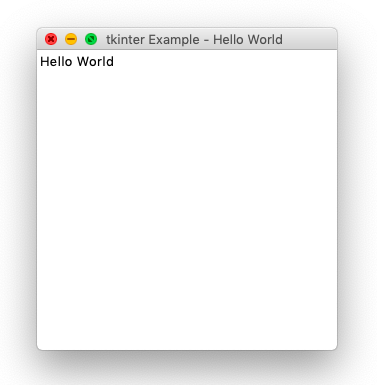
\includegraphics[width=0.8\textwidth]{images/HelloWorldGUI.png} 
	\caption{Hello World Beispiel mit grafischer Benutzeroberfl�che}
	\label{fig:HelloWorldGUI}
\end{figure}

Das Programm wird nun solange ausgef�hrt und bleibt in der Ereignisschleife, bis das Fenster geschlossen wird.
In dieser Schleife werden nicht nur Events wie Nutzereingaben (z.B. Mausklicks oder Tastatureingaben)
verarbeitet, sondern auch die des Fenstersystems (z.B. Redraw-Ereignisse und Fenster-Konfigurationsmeldungen) und
Ereignisse von Tkinter selbst.

\section{Die Layout-Manager}
\label{ui:layoutManager:section:dieLayoutManager}

In diesem Kapitel werden die Layout- oder Gemeometrie-Manager von Tkinter behandelt.
Grunds�tzlich stehen drei verschiedene Layout-Manager zur Verf�gung:

\begin{itemize}
    \item Pack
    \item Grid
    \item Place
\end{itemize}

Layout-Manager dienen in erster Linie dazu, Widgets in einem Wurzel-Element zu regestrieren,
anzuordnen und darzustellen. Besonders die Anordnung durch Angabe von Position und Gr��e eines Widgets
wird durch die Layout-Manager stark vereinfacht.

Einem Wurzel-Element sollte immer nur ein Layout-Manager angeh�ngt werden.

\subsection{Pack}
\label{ui:layoutManager:subsection:pack}

Der Pack-Manager ist der am einfachsten zu verwendende Layout-Manager.
Hier werden Widgets in Zeilen oder Spalten (vertikal oder horizontal) 'gepackt' und durch Optionen wie
\lstinline$fill$ oder \lstinline$expand$ gesteuert.

Im Vergleich zu dem sehr �hnlichen Grid-Manager ist der Pack-Manager etwas eingeschr�nkt,
aber in einigen wenigen Situationen sinnvoller zu nutzen. Speziell wenn einfache
Widgets �bereinander oder nebeneinander angeordnet werden oder Inhalte eines Widgets das gesamte
�bergeordnete Widget ausf�llen sollen, wird der Pack-Manager bevorzugt.

Das folgende Beispiel soll die Effekte des Pack-Managers verdeutlichen:

\lstinputlisting[language=Python]{chapters/userInterface/src/GUI_PackExample.py}
\label{ui:layoutManager:lst:lstinputlisting:gui_packExample}

\begin{figure}[ht]
	\centering
	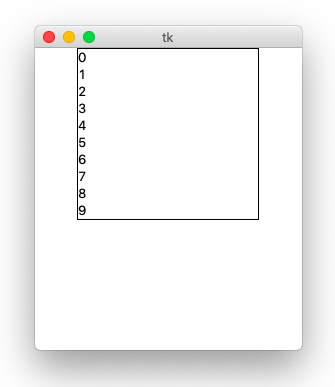
\includegraphics[width=0.5\textwidth]{images/PackManagerGUI_II.png}
	\caption{Listbox Widget mit einem Pack-Manager angeordnet}
	\label{ui:layoutManager:img:PackManagerGUI_II}
\end{figure}

Standardm��ig wird die Gr��e der Listbox so gew�hlt, dass zehn Elemente angezeigt
werden k�nnen. Im obigen Quelltext werden der Listbox allerdings doppelt so viele Elemente
�bergeben. Versucht der User nun das Wurzel-Element, sprich das Fenster, zu verg��ern,
um alle Elemente anzuzeigen, erzeugt Tkinter rund um das Listbox-Widget einen Abstand zum Fenster.
Um das Widget der gesamten zur Verf�gung stehenden Fl�che anzupassen, m�ssen die
Optionen \lstinline$fill$ und \lstinline$expand$ des Pack-Managers angesprochen werden.

\lstinputlisting[language=Python]{chapters/userInterface/src/GUI_PackExampleII.py}
\label{ui:layoutManager:lst:lstinputlisting:gui_packExampleII}

\begin{figure}[ht]
	\centering
	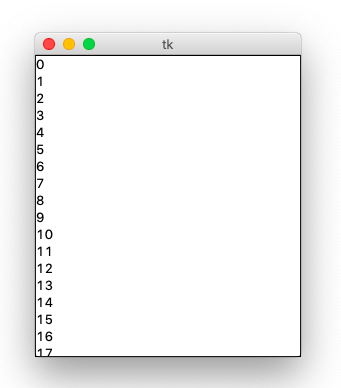
\includegraphics[width=0.5\textwidth]{images/PackManagerGUI_I.png}
	\caption{Listbox Widget mit einem Pack-Manager angeordnet unter Angabe von \lstinline$fill$ und \lstinline$expand$}
	\label{ui:layoutManager:img:PackManagerGUI_I}
\end{figure}

Die \lstinline$fill$-Option teilt dem Pack-Manager mit, dass der gesamte zur Verf�gung
stehende Raum durch das Widget ausgef�llt werden soll. Der dahinter stehende Wert
regelt wie der Raum gef�llt wird. \lstinline$BOTH$ bedeutet, dass das Widget
sowohl horizontal als auch vertikal expandieren soll.
Alternativ kann der Raum mit der Angabe \lstinline$X$ nur horizontal und mit der Angabe
\lstinline$Y$ nur vertikal ausgef�llt werden.

Dar�ber hinaus k�nnen Widgets mithilfe der Layout-Manager angeordnet werden.
Der Pack-Manager richtet Widgets, ohne weitere Angaben von Optionen, vertikal, sprich in Spalten aus.

\lstinputlisting[language=Python]{chapters/userInterface/src/GUI_PackExampleIII.py}
\label{ui:layoutManager:lst:lstinputlisting:gui_packExampleIII}

\begin{figure}[ht]
	\centering
	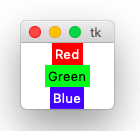
\includegraphics[width=0.3\textwidth]{images/PackManagerGUI_III.png}
	\caption{Mit Pack-Manager vertikal angeordnete Label-Widgets}
	\label{ui:layoutManager:img:PackManagerGUI_III}
\end{figure}

�ber die Option \lstinline$fill=X$ (horizontal) kann die Breite der Labels dem Eltern-Element angepasst werden.

\lstinputlisting[language=Python]{chapters/userInterface/src/GUI_PackExampleIV.py}
\label{ui:layoutManager:lst:lstinputlisting:gui_packExampleIV}

\begin{figure}[ht]
	\centering
	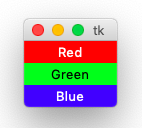
\includegraphics[width=0.3\textwidth]{images/PackManagerGUI_IV.png}
	\caption{Mit Pack-Manager vertikal angeordnete Label-Widgets unter Angabe von fill}
	\label{ui:layoutManager:img:PackManagerGUI_IV}
\end{figure}

Neben der vertikalen Ausrichtung der Labels ist auch eine horizontale m�glich, dazu steht
die \lstinline$side$-Option zur Verf�gung. Mit \lstinline$side=LEFT$ werden die
Widgets von links beginnend angeordnet. Weitere Paramter sind \lstinline$side=TOP$ (default),
\lstinline$side=BOTTOM$ und \lstinline$side=RIGHT$.

\subsection{Grid}
\label{ui:layoutManager:subsection:grid}

Der Grid-Manager ist der am flexibelsten einzusetzende Layout-Manager von Tkinter.
Besonders komfortabel ist der Einsatz bei dem Gestalten von Dialogfeldern. Die Handhabung
ist denkbar einfach. Das folgende Schaubild erl�utert die Aufteilung eines Gitterrasters:

\begin{figure}[ht]
	\centering
	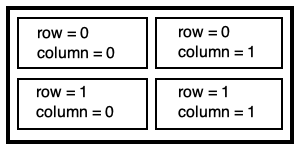
\includegraphics[width=0.4\textwidth]{images/GridManagerGUI.png}
	\caption{Gitterraster mit zwei Spalten und Reihen}
	\label{ui:layoutManager:img:GridManagerGUI}
\end{figure}

Nach dem Erzeugen eines Widget-Elements kann es �ber den Methoden-
Aufruf des Grid-Managers, unter Angabe von Zeilen und Spalten ausgerichtet
werden. Dabei muss weder H�he noch Breite der entsprechenden Zelle angegeben werden, der
Grid-Manager passt diese dem Content des Widgets an.

\lstinputlisting[language=Python]{chapters/userInterface/src/GUI_GridExampleI.py}
\label{ui:layoutManager:lst:lstinputlisting:gui_gridExampleI}

\begin{figure}[ht]
	\centering
	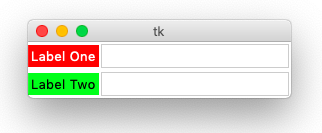
\includegraphics[width=0.5\textwidth]{images/GridManagerGUI_I.png}
	\caption{Mit Grid-Manager angeordnete Label- und Input-Widgets}
	\label{ui:layoutManager:img:GridManagerGUI_I}
\end{figure}

Leere Spalten und Zeilen werden von dem Layout-Manager ignoriert, das Ergebnis w�re
das selbe, wenn die Angabe anstelle von \lstinline$grid(row=0)$ und \lstinline$grid(row=1)$,
\lstinline$grid(row=5)$ und \lstinline$grid(row=10)$ lauten w�rde.

Der Inhalt der Zellen wird ohne weitere Angaben mittig angeordnet, was �ber die \lstinline$sticky$-Option
ge�ndert werden kann. Im Gegensatz zu der \lstinline$side$-Option des Pack-Managers,
nimmt \lstinline$sticky$ Himmelsrichtungen, also N, E, S und W als Angabe entgegen.
Mit \lstinline$Label(...).grid(row=0, sticky=W)$
beginnt der Text des Label-Widgets am linken Zellenrand (Westen). Auch Kombinationen wie beispielsweise
'unten links' (\lstinline$sticky=W+S$) sind m�glich.

\subsection{Place}
\label{ui:layoutManager:subsection:place}

Der dritte Layout-Manager von Tkinter ist der Place-Manager. Hier kann die Position und Gr��e eines
 Fensters explizit festgelegt werden, entweder absolut oder relativ zu einem anderen Fenster.
In der Regel werden Pack- oder Grid-Manager f�r die Gestaltung herk�mmlicher Dialog- und Fensteroberfl�chen
verwendet, in einigen wenigen F�llen ist jedoch der Place-Manager die bessere Wahl.
Beispielswei�e bei der Anordnung von Steuerelementen in Popup-Dialogen kommt der Place-Manager zum Einsatz.

Der Zugriff erfolgt wie bei ben vorherigen Layout-Managern �ber den Methodenaufruf unter Angabe
von X und Y - Koordinaten. Alternativ k�nnen mit der \lstinline$anchor$-Option �hnlich
der \lstinline$side$-Option des Pack-Managers, die Widgets �ber Kompass-Richtungen
ausgerichtet werden. Default ist NW (obere linke Ecke des Eltern-Elements).

\subsection{Zusammenfassung}
\label{ui:layoutManager:subsection:zusammenfassung}

Zusammenfassend kann gesagt werden:

\begin{itemize}
    \item Der Pack-Manger organisiert Widget-Elemente in Blocks. Anschlie�end werden diese im Eltern-Element platziert.
    \item Der Grid-Manger platziert Widget-Elemente in einer Tabellenartigen Struktur im Eltern-Element.
    \item Der Place-Manager platziert Widget-Elemente in spezifischer Position im Eltern-Element.
\end{itemize}

\uebung
\aufgabe{UI_aufgabe02}


\section{Widgets}
\label{ui:widgets:section:widgets}
Unter den Widgets werden in Tkinter alle grafischen Interaktionselemente wie Buttons, Labels,
Listboxes sowie Canvas etc. verstanden. Tkinter bietet hierf�r bereits vorgefertigte Klassen,
aus denen diese Widgets erzeugt werden k�nnen. Im Rahmen dieses Kapitels wird eine
Anwendung erstellt, die den Umgang mit einigen Widgets verdeutlichen soll und fortlaufend
dahingehend erweitert wird.

\subsection{Frame}
\label{ui:widgets:subsection:frame}
Frames fungieren, �hnlich wie die sogenannten divs in HTML, als Container um verschiedene
Widgets oder weitere Frames in einem bestimmten Bereich des Fensters zu gruppieren.
Dabei wird ein Rechteck erstellt und dem Eltern-Element �ber den Layout-Manager hinzugef�gt.

\subsection{Label}
\label{ui:widgets:subsection:label}
�ber Labels k�nnen im Userinterface einfache Textzeilen ausgegeben werden.
Diese lassen sich weiterhin auch dynamisch ver�ndern (z.B. bei einem Klick auf einen Button).

\subsection{Button}
\label{ui:widgets:subsection:button}
Mit dem Button hat der Nutzer die M�glichkeit mit dem Userinterface �ber einen Maus-Klick
zu interagieren. Buttons werden aus der Klasse \lstinline$Button$ erzeugt, dem Fenster oder Frame
bekannt gemacht und mit einem Text versehen. Zus�tzlich kann dem Button �ber \lstinline$command$
noch eine Funktion zugewiesen werden, die ausgef�hrt wird, sobald der Button gedr�ckt wurde.
In folgendem Beispiel wird bei Dr�cken des Buttons, in einem Label der Satz \lstinline$Hallo Python-World$
ausgegeben.

\lstinputlisting[language=Python]{chapters/userInterface/src/GUI_ButtonLabelExample.py}
\label{ui:widgets:lst:lstinputlisting:gui_buttonLabelExample}

\subsection{Entry}
\label{ui:widgets:subsection:entry}
�ber die sogenannten Entries lassen sich Eingaben vom Nutzer erfassen. Diese k�nnen dann im
Python-Skript weiterverarbeitet werden. Das vorherige Beispiel wird nun dementsprechend
erweitert, dass der Text, der bei Klick auf den Button ausgegeben wird, �ber \lstinline$get()$
vom Entry entgegen genommen wird.

\lstinputlisting[language=Python]{chapters/userInterface/src/GUI_EntryExample.py}
\label{ui:widgets:lst:lstinputlisting:gui_buttonLabelExample}

\subsection{Listbox}
\label{ui:widgets:subsection:listbox}
Um verschiedene Elemente in einer Liste anzeigen zu k�nnen bietet sich die Listbox an.
Der Text der vom Entry entgegengenommen wird soll nun einer solchen Listbox hinzugef�gt werden.
Dazu dient die Funktion \lstinline$insert()$. Der erste Parameter der �bergeben wird bestimmt
die Position in der Liste und der zweite das eigentliche Element.
Zus�tzlich wird der Anwendung ein zweiter Button hinzugef�gt um das jeweilig angew�hlte Element
der Listbox zu entfernen. Die Funktion \lstinline$curselection()$ gibt eine Liste der angew�hlten
Elemente zur�ck. Mithilfe von \lstinline$delete()$ wird dann das erste Element der zur�ckgegebenen Liste
aus der Listbox entfernt.

\lstinputlisting[language=Python]{chapters/userInterface/src/GUI_ListboxExample.py}
\label{ui:widgets:lst:lstinputlisting:gui_listboxwExample}

\subsection{Colorpicker}
\label{ui:widgets:subsection:colorpicker}

\subsection{Canvas}
\label{ui:widgets:subsection:canvas}

\uebung
\aufgabe{UI_aufgabe03}
\aufgabe{UI_aufgabe04}
\aufgabe{UI_aufgabe05}
\aufgabe{UI_aufgabe06}
\aufgabe{UI_aufgabe07}
\aufgabe{UI_aufgabe08}
\aufgabe{UI_aufgabe09}


% !TeX root = ../pythonTutorial.tex
\chapter{Python Bibliotheken}

\label{bibliotheken:numpy}
\section{NumPy}

NumPy ist eine Python-Bibliothek f�r wissenschaftliches Rechnen.
Sie beinhaltet unter anderem Folgendes:

\begin{itemize}
  \item m�chtige $n$-dimensionale Array-Objekte
  \item Werkzeuge zur Integration von C und Fortran
  \item Lineare Algebra, Fouriertransformation, Erzeugung von Zufallszahlen
\end{itemize}

% Zitat: http://www.numpy.org

Um NumPy zu installieren, kann der Befehl \lstinline!pip install numpy!
verwendet werden.

\subsection{Arrays}

Der Array-Datentyp von NumPy hei�t \lstinline!numpy.ndarray!. Anders als Pythons
Listentyp \lstinline!list! unterst�tzt \lstinline!numpy.ndarray! numerische
Operationen auf Arrays. Die Grundrechenarten werden zwischen zwei Arrays
elementweise und zwischen Array und \lstinline!int!/\lstinline!float! f�r alle
Elemente des Arrays durchgef�hrt.

So kann etwa jeder Wert in einem Array mit den folgenden Anweisungen um drei
erh�ht werden:
\begin{lstlisting}
import numpy as np
a = np.array([1,2,3])
a + 3 # [4 5 6]
\end{lstlisting}

Subtraktion, Multiplikation, Division, Ganzzahldivision und Potenzieren
funktionieren analog:\footnote{Der Import von \lstinline!numpy! wird der
�bersichtlichkeit halber nachfolgend ausgelassen.}
\begin{lstlisting}
a = np.array([1,2,3])
a - 3  # [-2 -1  0]
a * 3  # [3 6 9]
a / 3  # [0.33333333 0.66666667 1.        ]
a // 3 # [0 0 1]
a ** 3 # [ 1  8 27]
\end{lstlisting}

Zwei Arrays gleicher L�nge k�nnen elementweise miteinander verkn�pft werden:
\begin{lstlisting}
a = np.array([1,2,3])
b = np.array([4,5,6])
a + b  # [5 7 9]
a - b  # [-3 -3 -3]
a * b  # [ 4 10 18]
a / b  # [0.25 0.4  0.5 ]
a ** b # [  1  32 729]
a // b # [0 0 0]
\end{lstlisting}

Um ein NumPy-Array zu erzeugen, wird ein \lstinline!list!-Objekt an
\lstinline!np.array()! �bergeben, dabei wird der in der \lstinline{list}
enthaltene Datentyp in einem Datentyp von NumPy konvertiert. Um den Datentyp
eines Arrays herauszufinden, wird \lstinline!.dtype.name! genutzt. Anders
als bei \lstinline!list! m�ssen s�mtliche Elemente eines Arrays den gleichen
Typ haben.
\begin{lstlisting}
a = np.array([1,2,3])
a.dtype.name # 'int64'
b = np.array([1.4,2.5,3.6])
a.dtype.name # 'float64'
\end{lstlisting}

Wenn \lstinline!int! und \lstinline!float! gemischt �bergeben werden,
konvertiert NumPy in den Flie�kommatyp. Wie viele Bit f�r einen Integer bzw. ein
Float zur Verf�gung stehen, ist von der Prozessorarchitektur abh�ngig. Moderne
Computer unterst�zten in der Regel eine Gr��e von 64 Bit.


\subsection{Konstanten und Funktionen}
Es stehen f�r die mathematische Anwendungen auch Konstanten zur Verf�gung,
darunter die Folgenden mit den entsprechenden Werten und Pr�zisionen mit
\lstinline!float64!:
\begin{lstlisting}
>>> np.pi
3.141592653589793
>>> np.e
2.718281828459045
>>> np.euler_gamma
0.5772156649015329
>>> np.PINF
inf
>>> np.NINF
-inf
>>> np.NAN
nan
>>> np.PZERO
0.0
>>> np.NZERO
-0.0
>>> np.NAN
nan
\end{lstlisting}

\lstinline!np.NZERO! steht f�r die negative Darstellung der Null bei
Flie�kommazahlen, \lstinline!np.PZERO! f�r die positive Darstellung.

NumPy unterst�tzt eine Vielzahl an mathematischen Funktionen, darunter unter
anderem trigonometrische Funktionen, Rundungs-,
Summations- und Multiplikationsfunktionen und Funktionen zur Behandlung
komplexer Zahlen.

Die grundlegenden trigonometrischen Funktionen sind selbsterkl�rend, sie werden
elementweise auf das Array angewendet:
\begin{lstlisting}
>>> a = np.array([0, np.pi/6, np.pi/4, np.pi/3, np.pi/2])
>>> np.sin(a)
[0.         0.5        0.70710678 0.8660254  1.        ]
>>> np.cos(a)
[1.00000000e+00 8.66025404e-01 7.07106781e-01 5.00000000e-01
6.12323400e-17]
>> np.tan(a)
[0.00000000e+00, 5.77350269e-01, 1.00000000e+00,
1.73205081e+00, 1.63312394e+16]
\end{lstlisting}

Auch die Umrechung von Radians in Grad
\begin{lstlisting}
>>> a = np.array([0, np.pi/6, np.pi/4, np.pi/3, np.pi/2])
>>> np.degrees(a)
[ 0., 30., 45., 60., 90.]
\end{lstlisting}
und Grad in Radians m�glich:
\begin{lstlisting}
>>> a = np.array([ 0, 30, 45, 60, 90])
>>> np.radians(a)
[0.         0.52359878 0.78539816 1.04719755 1.57079633]
\end{lstlisting}

Mit \lstinline!np.around! k�nnen s�mtliche Werte im Array auf eine bestimmte
Anzahl von Stellen gerundet werden. Ohne Angabe eines zweiten Arguments wird
kaufm�nnisch auf die n�chste Ganzzahl gerundet.
\begin{lstlisting}
>>> a = np.array([1.49, 1.5, 1.51])
>>> np.round(a)
[1. 2. 2.]
\end{lstlisting}
Mit dem optionalen zweiten Argument wird die Anzahl an Nachkommastellen, auf die
gerundet werden soll, angegeben:
\begin{lstlisting}
>>> a = np.array([1.25, 1.53, 1.99])
>>> np.round(a, 1)
[1.2, 1.5, 2. ]
\end{lstlisting}

Um alle Elemente eines Arrays aufzusummieren, wird die Funktion \\
\lstinline!np.sum()! verwendet.
\begin{lstlisting}
>>> a = np.array([1, 2, 3])
>>> np.sum(a)
6
\end{lstlisting}
Mit \lstinline!np.prod()! k�nnen die Elemente der Liste miteinander
multipliziert werden.
\begin{lstlisting}
>>> a = np.array([2, 3, 4])
>>> np.prod(a)
24
\end{lstlisting}


Sollten \lstinline!nan! (not a number) im Array vorkommen k�nnen, so kann
\lstinline!np.nansum! beziehungsweise \lstinline!np.nanprod! verwendet werden.
Bei \lstinline!np.nansum! werden \lstinline!nan! als \lstinline!0!
interpretiert,
\begin{lstlisting}
>>> a = np.array([np.NAN, 1, 2, 3])
>>> np.sum(a)
nan
>>> np.nansum(a)
6.0
\end{lstlisting}
bei \lstinline!np.nanprod! als \lstinline!1!:
\begin{lstlisting}
>>> a = np.array([np.NAN, 2, 3, 4])
>>> np.prod(a)
nan
>>> np.nanprod(a)
24.0
\end{lstlisting}
Das Ergebnis der Addition bzw. Multiplikation ist vom Typ \lstinline!float64!.
\lstinline!nan! ist ein valider Flie�zahlwert, daher werden die restlichen Werte
in der zu konvertierenden \lstinline!list! von \lstinline!int! zu
\lstinline!float64! umgewandelt.



% !TeX root = ../pythonTutorial.tex
\chapter{Weiterf�hrende Themen}
% !TeX root = ../../pythonTutorial.tex
\section{Collections}
\label{collections}

In Python 3 existieren nativ die vier Datenstrukturen List, Tuple, Set und Dictionary, welche im Folgenden vorgestellt werden.

\subsection{List}
\label{collections:list}
Die Datenstruktur List bietet einen geordneten und ver�nderbaren Beh�lter f�r Python-Objekte, der Duplikate von Elementen erlaubt. Da eine List immer sortiert ist, k�nnen einzelne Elemente aus der Datenstruktur �ber den entsprechenden Index ausgew�hlt und ver�ndert werden. Python unterst�tzt intern keine Arrays, alternativ hierzu kann eine List verwendet werden.

Eine List kann wie folgt initialisiert werden:
\lstinputlisting[language=Python]{chapters/sections/listings/list/ListInit.py}
\label{collections:lst:listinit}

Dabei kann sie jegliche Art von Objekten beinhalten; der Datentyp spielt hierbei keine Rolle. 

Beispiel:
\lstinputlisting{chapters/sections/listings/list/ListDataType.py}
\label{collections:lst:listdatatype}

Im Gegensatz zu Java und C++ muss der Programmierer darauf achten und sicherstellen, dass die Datenstruktur mit Werten des entsprechenden Datentyps bef�llt wird, um Fehler aufgrund unterschiedlicher Datentypen zu vermeiden.

Der Inhalt einer List kann �ber die \lstinline$print()$-Methode ausgegeben werden. Im folgenden Beispiel werden verschiedene Elemente der List auf der Konsole ausgegeben.
Wird die List als Parameter gew�hlt, wird der Inhalt ausgegeben.
\lstinputlisting{chapters/sections/listings/list/ListPrint.py}
\label{collections:lst:listprint}

Wie zuvor erw�hnt, �hnelt die Verwaltung einer List der eines Arrays aus Java oder C++. Durch die Verwendung eines Index k�nnen einzelne Elemente ausgew�hlt oder ver�ndert werden.
\lstinputlisting{chapters/sections/listings/list/ListIndex.py}
\label{collections:lst:listindex}

Python erlaubt die Nutzung von negativen Indizes. Mit diesen kann der Inhalt der List in umgekehrter Reihenfolge ausgegeben werden. Ein Index von \lstinline$-1$ wird dem letzten Element der List zugeordnet, \lstinline$-2$ dem vorletzten.
\lstinputlisting{chapters/sections/listings/list/ListNegativeIndex.py}
\label{collections:lst:lsitnegativeindex}

In Python existiert f�r die Datenstruktur List keine Methode, die mit \lstinline$contains()$ in Java oder der \lstinline$find()$ aus C++ vergleichbar ist. Stattdessen stehen die Membership Operatoren \lstinline$in$ oder \lstinline$not in$ zur Verf�gung, welche auf eine beliebige Sequenz oder die hier beschriebenen Collections angewendet, Auskunft dar�ber gibt, ob das spezifizierte Element darin enthalten ist.
\lstinputlisting{chapters/sections/listings/list/ListInOperator.py}
\label{collections:lst:listinoperator}
    
Der Python Interpreter stellt nativ einige Funktionen zur Verf�gung. Eine davon ist die \lstinline$len()$-Methode, welche die Anzahl an Elementen in einem Objekt liefert.
\lstinputlisting{chapters/sections/listings/list/ListLen.py}
\label{collections:lst:listlen}
    
Das \lstinline$del$-Statement erlaubt das L�schen einzelner Elemente oder der gesamten List.
\lstinputlisting{chapters/sections/listings/list/ListDelete.py}
\label{collections:lst:listdel}
    

\subsubsection{Methoden einer List}
\label{collections:listmethodes}

\textbf{append():}
F�gt am Ende der List ein Objekt hinzu.
\lstinputlisting{chapters/sections/listings/list/ListAppend.py}
\label{collections:lst:listappend}

\textbf{clear():}
Entfernt s�mtliche Objekte aus der List.
\lstinputlisting{chapters/sections/listings/list/ListClear.py}
\label{collections:lst:listclear}

\textbf{copy():}
Liefert eine Kopie der List.
\lstinputlisting{chapters/sections/listings/list/ListCopy.py}
\label{collections:lst:listcopy}
    
%\newpage
\textbf{count():}
Liefert die Anzahl des spezifizierten Objekts in der List.
\lstinputlisting{chapters/sections/listings/list/ListCount.py}
\label{collections:lst:listcount}

\textbf{extend():} 
F�gt der \lstinline$liste1$ den Inhalt der \lstinline$liste2$ am Ende hinzu.
\lstinputlisting{chapters/sections/listings/list/ListExtend.py}
\label{collections:lst:listextend}
    
\textbf{index():}
Liefert den Index der Position, an der sich das erste spezifizierte Objekt in der List befindet.
\lstinputlisting{chapters/sections/listings/list/ListIndexMethode.py}
\label{collections:lst:listindexmethode}
    
\textbf{insert():}
F�gt ein Objekt an der gew�hlten Position der List hinzu.
\lstinputlisting{chapters/sections/listings/list/ListInsert.py}
\label{collections:lst:listinsert}

\textbf{pop():}
Entfernt das Objekt, das sich an der durch den Index spezifizierten Position befindet.
\lstinputlisting{chapters/sections/listings/list/ListPop.py}
\label{collections:lst:listpop}
    
\textbf{remove():}
Entfernt das erste Objekt der List, das der Spezifikation entspricht.
\lstinputlisting{chapters/sections/listings/list/ListRemove.py}
\label{collections:lst:listremove}
    
\textbf{reverse():}
Invertiert die Folge der Objekte in der List.
\lstinputlisting{chapters/sections/listings/list/ListReverse.py}
\label{collections:lst:listreverse}

\textbf{sort():}
Sortiert die List.
\lstinputlisting{chapters/sections/listings/list/ListSort.py}
\label{collections:lst:listsort}

    
\subsection{Tuple}
\label{collections:tuple}

Ein Tuple stellt einen geordneten und unver�nderbaren Beh�lter f�r Python-Objekte dar. Dieser erlaubt, wie eine List, Duplikate und den Zugriff auf einzelne Elemente �ber einen Index. Tuple sind Datenstrukturen, die ausschlie�lich gelesen werden k�nnen.

Ein Tuple wird mit folgender Syntax erzeugt:
\lstinputlisting{chapters/sections/listings/tuple/TupleInit.py}
\label{collections:lst:tupleinit}

Es ist m�glich, leere Tuple zu erzeugen. Wie zuvor erw�hnt, ist deren Inhalt unver�nderlich.

\subsubsection{Arbeiten mit einem Tuple}
\label{collections:workwithtuple} 

Der Inhalt eines Tuple kann, analog zur List, auf der Konsole ausgegeben werden. Das Zuweisen eines neuen Objekts mittels Index f�hrt im Gegensatz zur List zu einem Fehler.
\lstinputlisting{chapters/sections/listings/tuple/TupleIndex.py}
\label{collections:lst:tupleindex}    
    
Die Verwendung der Operatoren \lstinline$in$ und \lstinline$not in$ ist, wie die \lstinline$len()$-Methode, analog zur List-Datenstruktur.
\lstinputlisting{chapters/sections/listings/tuple/TupleInLen.py}
\label{collections:lst:tupleinlen} 
    
Das \lstinline$del$-Statement erlaubt das L�schen des Tuple. Aufgrund der Unver�nderbarkeit der Datenstruktur k�nnen keine einzelnen Elemente entfernt werden.
\lstinputlisting{chapters/sections/listings/tuple/TupleDelete.py}
\label{collections:lst:tupledelete}      

\subsubsection{Methoden eines Tuple}
\label{collections:tuplemethodes}

\textbf{count():}
Liefert die Anzahl des gew�hlten Werts in einem Tuple.
\lstinputlisting{chapters/sections/listings/tuple/TupleCount.py}    
\label{collections:lst:tuplecount}  

\textbf{index():}
Liefert die Position des ersten Werts, der mit dem spezifizierten Wert �bereinstimmt.
\lstinputlisting{chapters/sections/listings/tuple/TupleIndexMethode.py}
\label{collections:lst:tupleindexmethode}  

\subsection{Set}
\label{collections:set}
Ein Set ist durch das Hinzuf�gen oder Entfernen von Objekten ver�nderbar und erlaubt keine Duplikate. Das Initialisieren mit mehrfach identischen Werten f�hrt nicht zu einem Fehler, jedoch werden die �berz�hligen Werte aus dem Set entfernt. Die enthaltenen Elemente sind unver�nderlich. Zudem ist die Datenstruktur ungeordnet, weshalb nicht auf einzelne Objekte mittels Index zugegriffen werden kann. 

Ein Datenbeh�lter vom Typ Set kann mit folgender Syntax erzeugt werden:
\lstinputlisting{chapters/sections/listings/set/SetInit.py}
\label{collections:lst:setinit}  
    
\subsubsection{Arbeiten mit Sets}
\label{collections:workwithset}
Bei der Ausgabe eines Set auf der Konsole ist die Reihenfolge der Elemente zuf�llig. %TODO �berarbeiten NICHT ZUF�LLIG!

% TODO
% Wird der Inhalt eines Sets auf der Konsole ausgegeben, erscheint die Reihenfolge der Elemente willk�rlich, da diese nicht geordnet sind.
% Der Inhalt eines Sets ist nicht geordnet. Dies f�hrt zu einer willk�rlichen Reihenfolge der Elemente auf der Konsole. 
% "in"

Die Syntax f�r die Ausgabe auf der Konsole ist analog zur List. Die Verwendung eines Index ist nicht erlaubt und f�hrt zu einem Fehler.
\lstinputlisting{chapters/sections/listings/set/SetPrint.py}
\label{collections:lst:setprint} 
 
%\newpage
\subsubsection{Methoden eines Sets}
\label{collections:setmethodes} 

\textbf{add():}
F�gt dem Set ein Objekt hinzu.
\lstinputlisting{chapters/sections/listings/set/SetAdd.py}   
\label{collections:lst:setadd}  

\textbf{clear():}
Entfernt alle Elemente aus dem Set.
\lstinputlisting{chapters/sections/listings/set/SetClear.py}
\label{collections:lst:setclear}     

\textbf{copy():}
Liefert eine Kopie des Sets.
\lstinputlisting{chapters/sections/listings/set/SetCopy.py}
\label{collections:lst:setcopy}     

\textbf{difference():}
Liefert ein Set, das diejenigen Elemente enth�lt, die ausschlie�lich in \lstinline$setX$ vorkommen. Alle Element, die mit denen von \lstinline$setY$ �bereinstimmen, werden aus dem ersten entfernt. Alternativ ist dies auch �ber den Operator \lstinline$-$ m�glich.
\lstinputlisting{chapters/sections/listings/set/SetDifference.py}
\label{collections:lst:setdifference} 
    
\textbf{difference\_update():}
Entfernt diejenigen Elemente aus dem ersten Set, die mit denen aus dem zweiten �bereinstimmen.
\lstinputlisting{chapters/sections/listings/set/SetDifferenceUpdate.py}
\label{collections:lst:setdifferenceupdate}  
 
%\newpage
\textbf{discard():}
Entfernt das gew�hlte Element aus dem Set. Duplikate werden ebenfalls entfernt.
\lstinputlisting{chapters/sections/listings/set/SetDiscard.py}
\label{collections:lst:setdiscard} 

\textbf{intersection():}
Liefert ein Set mit der Schnittmenge zweier Sets. Alternativ ist dies auch mit der Angabe des \lstinline$&$-Operators m�glich.
\lstinputlisting{chapters/sections/listings/set/SetIntersection.py}
\label{collections:lst:setintersection} 

\textbf{intersection\_update():}
Entfernt alle Elemente, die sich nicht in der Schnittmenge beider Sets befinden.
\lstinputlisting{chapters/sections/listings/set/SetIntersectionUpdate.py}
\label{collections:lst:setintersectionupdate} 
    
\textbf{isdisjoint():}
Gibt Auskunft dar�ber, ob zwei Sets eine Schnittmenge besitzen. Liefert \lstinline$True$, wenn kein Element des ersten Sets im zweiten enthalten ist.
\lstinputlisting{chapters/sections/listings/set/SetIsDisJoint.py}
\label{collections:lst:setisdisjoint} 
    
\textbf{issubset():}
Gibt an, ob das gew�hlte Set eine Teilmenge enth�lt, die exakt dem ersten Set entspricht. Alternativ kann das Zeichen \lstinline$<$ verwendet werden.
\lstinputlisting{chapters/sections/listings/set/SetIsSubSet.py}
\label{collections:lst:setissubset} 
    
\textbf{pop():}
Entfernt ein beliebiges Element aus dem Set. Sollte das Set leer sein, wird ein Fehler generiert.
\lstinputlisting{chapters/sections/listings/set/SetPop.py}
\label{collections:lst:setpop} 
    
\textbf{remove():}
Entfernt das gew�hlte Element aus dem Set. Sollte das gew�hlte Element nicht in dem Set enthalten sein, wird ein Fehler angezeigt.
\lstinputlisting{chapters/sections/listings/set/SetRemove.py}
\label{collections:lst:setremove} 
    
\textbf{symmetric\_difference():}
Liefert ein Set, das die Vereinigung zweier Sets ohne deren Schnittmenge enth�lt.
\lstinputlisting{chapters/sections/listings/set/SetSymDiff.py}
\label{collections:lst:setsymdiff} 
    
\textbf{symmetric\_difference\_update():}
Vereinigt zwei Sets und entfernt deren Schnittmenge.%TODO
\lstinputlisting{chapters/sections/listings/set/SetSymDiffUpdate.py}
\label{collections:lst:setsymdiffupdate} 
    
\textbf{union():}
Liefert ein Set, das die Vereinigung zweier Sets darstellt. Duplikate werden entfernt.
\lstinputlisting{chapters/sections/listings/set/SetUnion.py}
\label{collections:lst:setunion} 
    
\textbf{update():}
F�gt einem Set die Items eines anderen hinzu. Duplikate werden entfernt.
\lstinputlisting{chapters/sections/listings/set/SetUpdate.py}
\label{collections:lst:setupdate} 
    
\subsubsection{Frozenset}

Im Gegensatz zu einem \glqq{}normalen\grqq{} Set kann ein Frozenset nicht mehr ver�ndert werden. Das Hinzuf�gen eines neuen Elements ist nicht erlaubt und f�hrt zu einem Fehler.
\lstinputlisting{chapters/sections/listings/set/SetFrozen.py}
\label{collections:lst:setfrozen} 

\subsection{Dictionary}
Ein Dictionary ist eine ungeordnete, ver�nderbare Datenstruktur, die keine Duplikate erlaubt und Schl�ssel-Objekt-Paare beinhaltet. Bei einer Ausgabe werden die Werte in zuf�lliger Reihenfolge ausgegeben, denn ein Dictionary besitzt keine Ordnung.

Ein Datenbeh�lter vom Typ Dictionary kann mit folgender Syntax erzeugt werden:
\lstinputlisting{chapters/sections/listings/dictionary/DictInit.py}

Demnach befindet sich hinter dem Schl�ssel \lstinline$k1$ das Objekt \lstinline$v1$ und analog dazu die weiteren Schl�ssel-Objekt-Paare. �ber den Schl�ssel \lstinline$k1$ l�sst sich auf das Objekt \lstinline$v1$ direkt zugreifen. Ebenso kann ein neues Objekt unter dem Schl�ssel \lstinline$k1$ zugewiesen werden.
\lstinputlisting{chapters/sections/listings/dictionary/DictPrint.py}

Eine alternative M�glichkeit, ein Dictionary zu erstellen, ist die Methode \lstinline$zip()$. Mit deren Hilfe kann aus zwei separaten List-Beh�ltern ein Dictionary generiert werden.
\lstinputlisting{chapters/sections/listings/dictionary/DictZip.py}

% TODO
% \subsubsection{Arbeiten mit Dictionaries}
% "in"
% Ausgaebe
% Values �ndern

%\newline 
\subsubsection{Methoden eines Dictionary}
\textbf{clear():}
Entfernt alle Eintr�ge aus dem Dictionary.
\lstinputlisting{chapters/sections/listings/dictionary/DictClear.py}

\textbf{copy():}
Liefert eine Kopie des Dictionary.
\lstinputlisting{chapters/sections/listings/dictionary/DictCopy.py}

\textbf{fromkeys():}
Liefert ein Dictionary mit den angegebenen Schl�sseln und Objekten.
\lstinputlisting{chapters/sections/listings/dictionary/DictFromKeys.py}

\textbf{get():}
Liefert das Objekt, das dem angegebenen Schl�ssel zugeordnet ist.
\lstinputlisting{chapters/sections/listings/dictionary/DictGet.py}

\textbf{items():}
Liefert eine List mit einem Tuple f�r jedes Schl�ssel-Objekt-Paar.
\lstinputlisting{chapters/sections/listings/dictionary/DictItems.py}

\textbf{keys():}
Liefert eine List von allen im Dictionary verwendeten Schl�sseln.
\lstinputlisting{chapters/sections/listings/dictionary/DictKeys.py}

\textbf{pop():}
Entfernt das Element mit dem entsprechenden Schl�ssel aus dem Dictionary und liefert das Objekt zur�ck.
\lstinputlisting{chapters/sections/listings/dictionary/DictPop.py}

\textbf{popitem():}
Liefert das zuletzt hinzugef�gte Schl�ssel-Objekt-Paar als Tuple und entfernt es aus dem Dictionary.
\lstinputlisting{chapters/sections/listings/dictionary/DictPopItem.py}

\textbf{setdefault():}
Liefert das dem Schl�ssel zugeordneten Objekt. Existiert dieser Schl�ssel nicht, wird ein neues Schl�ssel-Objekt-Paar mit dem angegebenen Schl�ssel und Objekt angelegt.
\lstinputlisting{chapters/sections/listings/dictionary/DictSetDefault.py}

\textbf{update():}
F�gt dem Dictionary ein Schl�ssel-Objekt-Paar hinzu.
\lstinputlisting{chapters/sections/listings/dictionary/DictUpdate.py}

\textbf{values():}
Liefert eine Liste mit allen im Dictionary enthaltenen Werten.
\lstinputlisting{chapters/sections/listings/dictionary/DictValues.py}

\subsection{Zusammenfassung}
In diesem Abschnitt wurde gezeigt, dass Python 3 uns mehrere Collections zur Aufbewahrung von Daten bereitstellt. Diese k�nnen je nach Datenstruktur unterschiedliche Eigenschaften aufweisen. W�hrend eine List die Daten sortiert vorh�lt und Duplikate zul�sst, werden bei einem Set entsprechende doppelte Eintr�ge vermieden. Betrachtet man das Set und seine Methoden genauer, ist dies der dahinter liegenden Mathematik, konkret der Mengenlehre geschuldet. Aus diesem Grund k�nnen alle g�ngigen mathematischen Operation auf Sets angewendet werden. Zum Schluss haben wir in diesem Abschnitt das Dictionary kennengelernt. Dieses ist �hnlich den Maps in Java. Dabei besteht ein Dictionary aus Schl�ssel-Objekt-Paaren, die hinter jedem Schl�ssel ein entsprechendes Objekt Mappen bzw. bereitstellen.




%
% Literatur
%
\cleardoublepage
\phantomsection
\addcontentsline{toc}{chapter}{Literaturverzeichnis}
\chaptermark{Literaturverzeichnis}
\sectionmark{Literatur}\label{literatur}
\bibliography{./bib/literatur}
%
% Anhang
%
\appendix

\chapter{L�sungshinweise}\label{solhinweise}
Hier finden sich die L�sungshinweise zu den Aufgaben.

\section{L�sungen zu Grundlagen}
\hinweis{grundlagen01}
\hinweis{grundlagen02}

\section{L�sungen zu Datentypen und Kontrollstrukturen}
\hinweis{DatatypesAufgabe1}
\hinweis{ifelseAufgabe1}
\hinweis{KontrollstrukturenAufgabe1}


\section{L�sungen zu Collections}
\hinweis{Collections/CollectionsAufgabe1List}
\hinweis{Collections/CollectionsAufgabe2List}
\hinweis{Collections/CollectionsAufgabe1Tuple}
\hinweis{Collections/CollectionsAufgabe2Tuple}
\hinweis{Collections/CollectionsAufgabe1Set}
\hinweis{Collections/CollectionsAufgabe1Dictionary}

\hinweis{testen01}
\hinweis{testen02} 
\hinweis{beispielAufgabe1}

\section{L�sungen zu Funktionen und Module}
\hinweis{functionsAndModules/01_greet}
\hinweis{functionsAndModules/02_greetMultiple}
\hinweis{functionsAndModules/03_getGeometryWithMostCorners}
\hinweis{functionsAndModules/04_pythagoras}
\hinweis{functionsAndModules/05_myMath}
\hinweis{functionsAndModules/06_myMath_2}


\section{L�sungen zu Benutzeroberfl�chen}
\hinweis{UI_aufgabe01}
\hinweis{UI_aufgabe02}
\hinweis{UI_aufgabe03}

\section{L�sungen zu Maschinelles Lernen}
\hinweis{machinelearning1}
\hinweis{machinelearning2}

\section{L�sungen zu Nebenl�ufigkeit}
\hinweis{nebenlaufigkeit01}
\hinweis{nebenlaufigkeit02}
\hinweis{nebenlaufigkeit03}
\hinweis{nebenlaufigkeit04}
\hinweis{nebenlaufigkeit05}
\hinweis{nebenlaufigkeit06}
\hinweis{nebenlaufigkeit07}
%
% Index
%\clearevenpage
%\phantomsection
%\small
%\chaptermark{Index}
%\sectionmark{Index}
%\printindex
%\normalsize
\end{document}
